\documentclass[UTF8,a4paper,zihao=-4,fontset=macnew]{ctexart}

\usepackage[
  top=2.5cm,
  right=2.5cm,
  bottom=2.5cm,
  left=3cm,
  headheight=15pt,
  headsep=0.45cm,
  footskip=0.72cm
]{geometry}
\usepackage{fontspec}
\usepackage{graphicx}
\usepackage{xcolor}
\usepackage{array}
\usepackage{tabularx}
\usepackage{makecell}
\usepackage{multirow}
\usepackage{enumitem}
\usepackage{fancyhdr}
\usepackage{listings}
\usepackage{hyperref}
\usepackage{amsmath}
\usepackage{anyfontsize}
\usepackage{microtype}
\usepackage{float}
\usepackage{booktabs}
\usepackage{longtable}
\usepackage[font=small]{caption}
\usepackage[font=footnotesize]{subcaption}
\usepackage{tikz}
\usetikzlibrary{arrows.meta, positioning, shapes.geometric, fit, backgrounds, calc, matrix}
\tikzset{
  blk/.style ={rectangle, rounded corners=2pt, draw, align=center, inner sep=4pt, font=\footnotesize},
  io/.style  ={rectangle, draw, align=center, inner sep=4pt, font=\footnotesize, fill=black!4},
  dec/.style ={diamond, draw, aspect=2.2, align=center, inner sep=1pt, font=\footnotesize},
  lyr/.style ={rectangle, draw, rounded corners=2pt, align=center, font=\footnotesize, fill=black!3},
  grp/.style ={rectangle, rounded corners=3pt, draw=black!35, dashed, inner sep=6pt},
  fl/.style  ={-{Latex[length=2mm]}, >=Latex},
  fl2/.style ={{Latex[length=2mm]}-{Latex[length=2mm]}},
  lbl/.style ={font=\scriptsize, fill=white, inner sep=1pt},
}

\setmainfont{Times New Roman}
\setsansfont{Arial}
\setmonofont{Menlo}

\hypersetup{hidelinks}
\setlength{\parindent}{2em}
\setlength{\parskip}{0pt}
\setlength{\emergencystretch}{3em}
\tolerance=2000
\hbadness=10000
\renewcommand{\arraystretch}{1.0}
\definecolor{deepblue}{RGB}{0,0,128}

\newcolumntype{C}[1]{>{\centering\arraybackslash}p{#1}}
\newcolumntype{L}[1]{>{\raggedright\arraybackslash}p{#1}}
\newcommand{\rednote}[1]{{\color{red}#1}}
\newcommand{\bluenote}[1]{{\color{blue}#1}}
\newcommand{\deepbluenote}[1]{{\color{deepblue}#1}}
\newcommand{\notepara}[2]{%
  {\setlength{\leftskip}{2em}\setlength{\parindent}{0pt}\color{#1}#2\par}%
}
\newcommand{\bluepara}[1]{\notepara{blue}{#1}}
\newcommand{\redpara}[1]{\notepara{red}{#1}}
\newcommand{\deepbluepara}[1]{\notepara{deepblue}{#1}}
\newcommand{\blankline}[1]{\makebox[#1]{\hrulefill}}
\newcommand{\ulfield}[2]{\vtop{\hbox{\makebox[#1][c]{#2}}\kern1.5pt\hrule height 0.4pt}}
\newcommand{\coverrow}[4]{%
  \noindent\makebox[2.0cm][l]{#1}\ulfield{#2}{#3}\makebox[#4]{}\\[0.42cm]%
}

\fancypagestyle{reporthead}{
  \fancyhf{}
  \fancyhead[L]{\zihao{-5}重庆理工大学综合课程设计报告}
  \fancyhead[R]{\zihao{-5}物联网工程专业-综合课程设计I-桌面用电监控}
  \renewcommand{\headrulewidth}{0.4pt}
  \renewcommand{\footrulewidth}{0pt}
}

\fancypagestyle{reportbody}{
  \fancyhf{}
  \fancyhead[L]{\zihao{-5}重庆理工大学综合课程设计报告}
  \fancyhead[R]{\zihao{-5}物联网工程专业-综合课程设计I-桌面用电监控}
  \fancyfoot[C]{\zihao{-5}\thepage}
  \renewcommand{\headrulewidth}{0.4pt}
  \renewcommand{\footrulewidth}{0pt}
}

\lstdefinelanguage{Rust}{
  keywords={fn,let,mut,pub,extern,crate,use,mod,struct,enum,impl,trait,type,const,static,if,else,while,for,loop,match,return,break,continue,as,in,ref,self,Self,super,where,unsafe,async,await,move,no_mangle,no_std,repr},
  sensitive=true,
  morecomment=[l]{//},
  morecomment=[s]{/*}{*/},
  morestring=[b]",
  morestring=[b]',
}

\lstdefinestyle{appendixcode}{
  basicstyle=\ttfamily\zihao{5},
  commentstyle=\color{black!55},
  breaklines=true,
  columns=fullflexible,
  keepspaces=true,
  showstringspaces=false,
  tabsize=4,
  xleftmargin=2em,
  aboveskip=0.5em,
  belowskip=0.5em
}
\lstdefinestyle{serialterm}{
  basicstyle=\ttfamily\zihao{-5},
  frame=single,
  framesep=4pt,
  breaklines=true,
  breakindent=2em,
  columns=fullflexible,
  keepspaces=true,
  xleftmargin=1em,
  xrightmargin=1em,
  aboveskip=0.5em,
  belowskip=0.5em
}

\newcommand{\tocline}[2]{%
  \noindent\makebox[\textwidth][l]{\heiti\bfseries #1\dotfill #2}\par\vspace{0.05cm}%
}
\newcommand{\tocsubline}[2]{%
  \noindent\hspace{0.72cm}\makebox[\dimexpr\textwidth-0.72cm\relax][l]{\heiti\bfseries #1\dotfill #2}\par\vspace{0.05cm}%
}
\newcommand{\sectiontitle}[2]{%
  \setcounter{section}{\numexpr#1-1\relax}\refstepcounter{section}%
  \vspace*{-0.32cm}%
  {\noindent\heiti\bfseries\fontsize{18pt}{20pt}\selectfont #1.\quad #2\par}%
  \vspace{0.50cm}%
}
\makeatletter
\def\@extractsubnum#1.#2\@nil{#2}
\newcommand{\subsectiontitle}[2]{%
  \setcounter{subsection}{\numexpr\@extractsubnum#1\@nil-1\relax}\refstepcounter{subsection}%
  \vspace{0.34cm}%
  {\noindent\heiti\bfseries\fontsize{16pt}{18pt}\selectfont #1.\quad #2\par}%
  \vspace{0.54cm}%
}
\newcommand{\subsubsectiontitle}[2]{%
  \vspace{0.24cm}%
  {\noindent\heiti\bfseries\fontsize{14pt}{16pt}\selectfont #1\quad #2\par}%
  \vspace{0.34cm}%
}
\makeatother
\newcommand{\itemline}[2]{%
  {\setlength{\leftskip}{2em}\setlength{\parindent}{0pt}%
  \noindent(#1)\quad #2\par}%
}
\newcommand{\blueitemline}[2]{%
  {\setlength{\leftskip}{2em}\setlength{\parindent}{0pt}\color{blue}%
  \noindent(#1)\quad #2\par}%
}
\newcommand{\spacedblueitemline}[2]{%
  \blueitemline{#1}{#2}\vspace{0.88cm}%
}
\newcommand{\lineblueitemline}[2]{%
  \blueitemline{#1}{#2}\vspace{0.18cm}%
}

\begin{document}

% Page 1: cover.
\thispagestyle{empty}
\zihao{5}
\noindent
{\setlength{\tabcolsep}{2pt}
\begin{tabular}{|C{1.65cm}|C{3.80cm}|C{3.80cm}|}
\hline
\multicolumn{3}{|c|}{\heiti 总成绩(30 分)}\\
\hline
\multirowcell{2}{\heiti 项目} & \heiti 通讯协议实现及分析 & \heiti 报告质量及团队协作\\
 & \heiti 15 分 & \heiti 15 分\\
\hline
\heiti 得分 & & \\
\hline
\heiti 评分人 & \multicolumn{2}{c|}{}\\
\hline
\end{tabular}
}

\vspace{1.20cm}
\begin{center}
  
\includegraphics[width=10.4cm]{figures/cqut-logo-wordmark.png}

  \vspace{1.35cm}
  {\heiti\bfseries\zihao{-0} 综合课程设计I 报告\par}

  \vspace{1.05cm}
  {\heiti\zihao{3}题目：\quad \ulfield{8.0cm}{桌面用电监控设计实现}\par}

  \vspace{1.65cm}
  \begin{minipage}{9.8cm}
    \zihao{4}\raggedright
    \coverrow{二级学院}{7.0cm}{计算机科学与工程学院}{0pt}
    \coverrow{专\qquad 业}{7.0cm}{物联网工程}{0pt}
    \coverrow{班\qquad 级}{7.0cm}{}{0pt}
    \noindent 学生姓名\ulfield{3.0cm}{}学号\ulfield{2.9cm}{}\\[0.42cm]
    \coverrow{指导教师}{7.0cm}{}{0pt}
    \coverrow{时\qquad 间}{7.0cm}{2026.6}{0pt}
  \end{minipage}
\end{center}

\clearpage

% Page 3: abstract.
\pagenumbering{Roman}
\setcounter{page}{1}
\thispagestyle{empty}
\setlength{\parindent}{2em}
\phantomsection\label{sec:abstract}
\vspace*{\fill}
\begin{center}
\begin{minipage}{0.85\textwidth}
\begin{center}
{\heiti\zihao{4} 摘\quad 要}
\end{center}
\vspace{0.45cm}
\zihao{-4}
\setlength{\parindent}{2em}

本课程设计基于 STM32F103RCT6 微控制器，设计并实现了一套桌面用电监控系统。系统采用无操作系统的裸机前后台轮询结构，软件采用模块化设计：利用 PWM 输出产生测试频率，通过定时器输入捕获功能测量频率，使用双通道 DAC 生成测试正弦波，并对三通道 ADC 的交流信号进行准同步顺序扫描采样与电参量计算；本地显示采用 TFT LCD 多级菜单，远程通信则通过 USART 二进制帧协议实现。

系统以 MiniSTM32 开发板为核心硬件平台。在信号生成与感知部分，利用 PA8/TIM1 输出占空比为 50\% 且频率可调的方波，并通过 PA1/TIM2 的输入捕获功能测量外部信号频率；利用 PA4/PA5 DAC 通道配合 DMA 循环搬运，输出 128 点的正弦波信号。在交流信号采集方面，PC0/PC3/PC2 三通道 ADC 由 TIM3 触发，以 6400 Hz 的采样率对电压、电流和漏电电流进行顺序扫描采样。三路通道共用同一触发源，其间转换时差极小，对于 50 Hz 基波信号的电参量计算影响可以忽略。采样数据由 DMA 传输至工作缓冲区后，程序调用整型算法计算电压与电流有效值、有功功率、视在功率及功率因数。通信协议采用分层设计，传输层以 A5 5A 帧头与 CRC-16/Modbus 校验保障传输可靠性，命令层则在帧内承载 ASCII 文本指令(支持 HELP、STATUS?、REPORT ON/OFF、PWM SET、DAC SET 等命令)。人机交互界面通过多页面状态机实现，包含仪表盘首页、测试菜单与四个功能子页面，且 LCD 显示与串口查询共享同一套全局状态数据，以确保两端显示数据的一致性。

系统调试表明，频率测量分辨率达到 0.01 Hz，PWM 设定范围为 1--100000 Hz，DAC 双通道频率在 1--1000 Hz、幅度在 0--2047 内均可独立调节。在系统联调测试下，ADC 采样、电参量计算、显示刷新及串口通信等模块均运行稳定，实现了课程设计的各项功能要求。

\vspace{1.55cm}
\noindent{\heiti 关键词：}STM32F103；ADC 采样；二进制帧协议；整型电参量计算
\end{minipage}
\end{center}
\vfill
\clearpage

% Page 6: manual table of contents.
\thispagestyle{reporthead}
\vspace*{0.45cm}
\begin{center}
{\heiti\zihao{3} 目\quad 录}
\end{center}
\vspace{0.58cm}
\zihao{5}
\setlength{\parindent}{0pt}
\tocline{摘\quad 要}{\pageref{sec:abstract}}
\tocline{1. 课程设计的目的及要求}{\pageref{sec:purpose}}
\tocsubline{1.1. 课程设计目的}{\pageref{sec:purpose-goal}}
\tocsubline{1.2. 课程设计要求}{\pageref{sec:purpose-req}}
\tocline{2. 系统分析}{\pageref{sec:analysis}}
\tocsubline{2.1. 系统需求与功能边界}{\pageref{sec:analysis-function}}
\tocsubline{2.2. 系统性能指标}{\pageref{sec:analysis-performance}}
\tocsubline{2.3. 设计约束}{\pageref{sec:analysis-algorithm}}
\tocline{3. 系统设计}{\pageref{sec:design}}
\tocsubline{3.1. 系统整体设计}{\pageref{sec:design-system}}
\tocsubline{3.2. 硬件设计}{\pageref{sec:design-hardware}}
\tocsubline{3.3. 软件设计}{\pageref{sec:design-software}}
\tocsubline{3.4. 通信协议设计}{\pageref{sec:protocol-design}}
\tocline{4. 频率测量}{\pageref{sec:frequency}}
\tocsubline{4.1. 测试频率生成}{\pageref{sec:frequency-generate}}
\tocsubline{4.2. 频率测量}{\pageref{sec:frequency-measure}}
\tocsubline{4.3. 通信协议}{\pageref{sec:frequency-protocol}}
\tocline{5. 交流 ADC 采样}{\pageref{sec:adc}}
\tocsubline{5.1. 测试电压电流生成与实际信号来源}{\pageref{sec:adc-generate}}
\tocsubline{5.2. 信号采集}{\pageref{sec:adc-sampling}}
\tocsubline{5.3. 通信协议}{\pageref{sec:adc-protocol}}
\tocsubline{5.4. 波形曲线绘制}{\pageref{sec:adc-waveform}}
\tocline{6. 电参量计算与分析}{\pageref{sec:calculation}}
\tocsubline{6.1. 交流电参量计算方法}{\pageref{sec:calculation-method}}
\tocsubline{6.2. 程序实现}{\pageref{sec:calculation-program}}
\tocsubline{6.3. 通信设计}{\pageref{sec:calculation-comm}}
\tocline{7. 系统调试}{\pageref{sec:debug}}
\tocsubline{7.1. 通信协议测试}{\pageref{sec:debug-protocol}}
\tocsubline{7.2. 频率调试}{\pageref{sec:debug-frequency}}
\tocsubline{7.3. AD 采样调试}{\pageref{sec:debug-ad}}
\tocsubline{7.4. 电参量调试}{\pageref{sec:debug-calculation}}
\tocsubline{7.5. 联机调试}{\pageref{sec:debug-online}}
\tocline{8. 总结与展望}{\pageref{sec:summary}}

\clearpage

\pagestyle{reportbody}
\pagenumbering{arabic}
\zihao{5}
\setlength{\parindent}{2em}
\setlength{\baselineskip}{20pt}

% ==============================
% 第 1 章：课程设计的目的及要求
% ==============================
\vspace*{0.18cm}
\sectiontitle{1}{课程设计的目的及要求}
\phantomsection\label{sec:purpose}

本课程设计以桌面用电监控为主题，基于 STM32F103RCT6 微控制器开发板设计并实现了一套嵌入式监控系统，具备信号发生与采集、电参量计算、本地显示及远程通信功能。整个设计过程涵盖了硬件接口配置、外设驱动编写、通信协议设计、算法实现与人机交互界面开发，旨在通过完整的系统级工程实践，锻炼嵌入式系统开发能力。

\subsectiontitle{1.1}{课程设计目的}
\phantomsection\label{sec:purpose-goal}
\itemline{1}{了解并熟悉常用电子元器件工作原理和功能特性。}
\itemline{2}{信号感知电路数据：掌握交流电压、电流检测电路，继电器控制方法。}
\itemline{3}{开发平台及工具使用：熟练运用 Keil MDK 软件进行单片机的 C 语言编程。}
\itemline{4}{通信及通信协议：掌握串行通讯简单协议的程序设计思想和实现。}
\itemline{5}{频率信号生成与感知：掌握基于 PWM 的频率波形生成与基于定时器捕捉功能的频率测量的程序设计思想和实现。}
\itemline{6}{正弦波信号生成：掌握基于 DMA 传送的 DA 双路带幅值、相位调整的正弦波生成方法与实现。}
\itemline{7}{交流信号采集：掌握基于定时启动、DMA 传送的 AD 转换程序设计与实现。}
\itemline{8}{交流波形绘制：掌握交流电压、电流 LCD 屏幕绘制程序设计。}
\itemline{9}{信号分析：掌握交流电参量计算算法与程序实现。}
\itemline{10}{培养嵌入式系统设计、分析及展示能力。}

\subsectiontitle{1.2}{课程设计要求}
\phantomsection\label{sec:purpose-req}
\itemline{1}{仔细阅读课程设计指导书，分析桌面用电电路原理；}
\itemline{2}{利用 AI 帮助分析设计原理、步骤、实现；}
\itemline{3}{设计频率测试信号；}
\itemline{4}{设计修改频率测试信号参数通信协议；}
\itemline{5}{设计频率测量程序；}
\itemline{6}{设计用于交流电压电流模拟测试信号；}
\itemline{7}{设计修改交流电压电流模拟测试信号参数通信协议；}
\itemline{8}{设计交流采样程序；}
\itemline{9}{曲线绘制；}
\itemline{10}{设计电参量计算算法及程序；}
\itemline{11}{串行通讯协议设计及串口助手调试显示；}
\itemline{12}{系统联调；}
\itemline{13}{系统答辩；}
\itemline{14}{系统设计过程中相互交流、团队协作及其总结；}
\itemline{15}{设计总结。}

\clearpage

% ==============================
% 第 2 章：系统分析
% ==============================
\sectiontitle{2}{系统分析}
\phantomsection\label{sec:analysis}

本系统的核心任务是生成、采集、计算并展示桌面用电环境中的各种电信号。系统以 STM32F103RCT6 微控制器为主控，通过协调定时器、DAC、ADC、DMA 和 USART 等片上外设，实现了测试信号发生、信号频率测量、交流信号采样、电参量整型计算以及远程串口通信等功能。本章将对系统的功能设计、性能指标要求以及核心计算算法展开分析。

\subsectiontitle{2.1}{系统需求与功能边界}
\phantomsection\label{sec:analysis-function}

本系统旨在实现对桌面用电环境中关键电学参数的实时监控、分析展示与远程调试。为了实现这一目标，系统需要支持信号的发生、采集、处理及通信。根据实际部署与架构分工，系统的功能边界划分为微控制器控制端、硬件前级信号调理端以及上位机监测端。

\itemline{1}{核心功能需求}

系统的核心功能需求主要包括以下五个方面：
\begin{itemize}
  \item \textbf{测试信号发生需求：} 系统需要能够自主产生高精度的测试信号，用于在没有实际交流市电输入时，对系统的采集与计算链路进行闭环自检。具体包括产生占空比固定的方波信号（PWM），以及幅值、频率和相位可调的双通道正弦波信号（DAC）。
  \item \textbf{电学信号测量需求：} 系统必须能够精确测量输入信号的频率，包括测试方波的自检测频以及电网市电频率的实时检测。
  \item \textbf{用电数据采集需求：} 系统需要对用电环境中的关键交流信号进行同步、连续的数据采集，包括负载电压信号、负载电流信号以及异常情况下的漏电电流信号。
  \item \textbf{本地可视化与交互需求：} 现场终端需要提供直观的人机交互界面，以便现场人员查看实时的电压电流波形、各电参量（有效值、功率、功率因数等）以及修改测试参数。
  \item \textbf{远程通信与在线调试需求：} 监控终端应具备与上位机或网关的通信能力，支持以远程方式下发配置命令（查询状态、修改参数、控制继电器）和接收终端周期性自动上报的监控参数。
\end{itemize}

\itemline{2}{功能边界划分}

本系统的功能在硬件和软件实体间做出了清晰的划分，以降低系统耦合度，提高整体可靠性：
\begin{itemize}
  \item \textbf{微控制器控制端（STM32 主控）：} 负责核心业务的逻辑调度，控制片上定时器、DAC 及 ADC 完成信号发生与数据采集；在本地执行无浮点运算的定点数电参量算法；驱动 TFT LCD 屏幕渲染状态波形与多级菜单交互；接收并解析来自串口的二进制通信帧，维护系统运行状态。
  \item \textbf{硬件前级信号调理端（miniIO 副板）：} 负责高压用电环境与微控制器之间的安全隔离与信号调理。使用电压与电流互感器隔离高压市电，将双极性的交流大信号等比例缩小并进行低通滤波；利用 1.65 V 参考电压源对信号进行直流偏置抬升，将双极性交流信号转化为 0--3.3 V 的安全单极性信号以适配主控 ADC 通道；同时将交流市电进行整形转化为低压方波以供主控测量电网频率；提供继电器控制电路以便主控通过 GPIO 引脚安全控制强电通路。
  \item \textbf{上位机监测端（PC 测试工具）：} 负责系统的远程状态管理与调试。通过串口发送符合协议帧规范的控制命令，对终端状态及参数进行全量轮询，或直接监听终端主动推送的事件帧，解析出参数并在上位机端直观呈现。
\end{itemize}

\subsectiontitle{2.2}{系统性能指标}
\phantomsection\label{sec:analysis-performance}

为了保证桌面用电监控系统的精度、实时性及人机交互的流畅度，本设计在各功能模块上制订了明确的性能指标要求：

\itemline{1}{信号发生指标}
\begin{itemize}
  \item \textbf{测试方波信号（PWM）：} PA8 通道输出 50\% 固定占空比方波测试信号，其频率调节范围为 1 Hz 至 100 kHz，频率设置分辨率为 1 Hz。
  \item \textbf{测试正弦波信号（DAC）：} PA4/PA5 通道独立输出单/双路正弦波信号，频率调节范围为 1 Hz 至 1000 Hz，幅度码值调节范围为 0--2047（对应 0--3.3 V 满幅），初始相位调节范围为 0--359 度。
\end{itemize}

\itemline{2}{采样与测量指标}
\begin{itemize}
  \item \textbf{频率测量：} 测频模块支持输入信号周期时间捕获，测频分辨率需达到 0.01 Hz。对于 50 Hz 左右电网信号，周期时间捕获误差需限制在 $\pm$1 $\mu$s 内。
  \item \textbf{模拟通道采集（ADC）：} 规则采样组支持对电压、电流和漏电三路调理信号进行顺序扫描采集，单通道采样分辨率为 12 位（码值 0--4095）。系统采样率设定为 6400 Hz。针对 50 Hz 交流电，单周期采样样点数需精确达到 128 点，以满足电参量 RMS 全周期离散积分计算对 Nyquist 定理及同步采样的要求。
\end{itemize}

\itemline{3}{分析与显示指标}
\begin{itemize}
  \item \textbf{电参量测量分辨率：} 为确保测量精度与直观展现，电参量的最终数字显示分辨率设计为：交流有效电压 0.01 V、交流有效电流 0.001 A、有功功率 0.1 W。
  \item \textbf{本地屏幕刷新：} LCD 显示界面的波形绘制应视觉平稳、无明显闪烁。Dashboard 主监测页面的刷新率定为约 3 Hz（由 ADC 的第 17 个新帧中断事件驱动更新）；菜单切换及参数更新的响应延迟需小于 100 ms。
  \item \textbf{远程通信速率：} 通信串口波特率配置为 115200 bps，自动上报周期为固定间隔约 1 s。
\end{itemize}

\subsectiontitle{2.3}{设计约束}
\phantomsection\label{sec:analysis-algorithm}

为确保桌面用电监控系统在各种工况下能够安全、可靠地不间断运行，系统在硬件、软件以及运行时间上面临以下设计约束：

\itemline{1}{硬件与计算资源约束}
\begin{itemize}
  \item \textbf{无浮点协处理器（No FPU）：} 主控芯片 STM32F103RCT6 搭载 Cortex-M3 核心，不具备硬件浮点运算单元。为保证系统调度的实时性，核心算法（包括正弦波缩放与交流电参量 RMS 计算等）必须全部采用定点数及整型算术运算实现，严禁引入耗时的浮点运算。
  \item \textbf{静态存储约束：} 考虑到嵌入式系统的长期运行稳定性，软件架构设计约束为不允许动态内存分配（禁用堆空间），所有的缓冲区、状态结构体及通信队列均须在编译期作为静态全局变量分配在 RAM 中。
\end{itemize}

\itemline{2}{信号电气安全约束}
\begin{itemize}
  \item \textbf{ADC 电压安全输入约束：} 微控制器内置的 ADC 转换通道能够接收的电压范围为 0--3.3 V。然而交流市电信号是具有正负半周的双极性信号，直接接入将导致芯片烧毁。因此，前级调理电路必须施加 1.65 V 的直流偏置抬升，软件计算算法亦必须以该中点电压基线作为依据，通过数字去直流（de-biasing）处理还原出真实的交流波形。
\end{itemize}

\itemline{3}{实时性与通信时序约束}
\begin{itemize}
  \item \textbf{算法实时计算约束：} 交流电参量积分计算以网频交流周期为单位进行。算法必须在当前周期采样缓冲区填满的极短时间内（在下一次采样触发前）完成去直流、累加平方和及开方计算，防止数据搬运阻塞与缓冲区溢出。
  \item \textbf{串口通信鲁棒性约束：} 串口数据流解析基于接收中断及环形缓冲区。为防止不完整的脏包或因噪声造成的半帧导致解析器死锁，系统需引入半帧间隔超时保护（限制在 300 ms 内），且当检测到协议帧头或校验失败时能立即自动重置解析状态。
\end{itemize}

\clearpage

% ==============================
% 第 3 章：系统设计
% ==============================
\sectiontitle{3}{系统设计}
\phantomsection\label{sec:design}

本章介绍系统整体架构、硬件接口分配与软件模块设计。

\subsectiontitle{3.1}{系统整体设计}
\phantomsection\label{sec:design-system}

系统主控采用 STM32F103RCT6 微控制器。系统上电后，引导程序和初始化函数会依次配置板级外设安全电平、初始化 LCD 屏、按键输入接口、串口通信协议栈、配置测频与 PWM 发生相关定时器、以及 DAC、ADC 和 UI 菜单状态机，准备就绪后进入系统调度主循环。

主循环以轮询机制按固定顺序调度各功能任务，执行流程包括：获取微秒级统一系统时间戳、解析串口数据并分发指令、处理测频超时与事件节流、读取 ADC 双缓冲并调用算法计算电参数、处理状态周期性上报、扫描按键并驱动菜单状态机、读取全局状态数据，以及刷新 LCD 显示。每一轮调度循环均基于同一次获取的时间戳 \texttt{now\_us}，从而避免了多模块调度过程中的时序冲突与数据源不一致。

% [占位图]
\begin{figure}[H]
\centering
\begin{subfigure}[b]{\textwidth}
\centering
\resizebox{\linewidth}{!}{%
\begin{tikzpicture}[node distance=6mm and 9mm]
  \node[io] (mains) {市电输入\\/ 负载};
  \node[blk, right=of mains] (mini) {miniIO 副板\\信号处理\\电压/电流/漏电/频率};
  \node[blk, right=of mini] (jp1) {JP1\\排针};
  \node[blk, minimum height=16mm, right=of jp1] (mcu) {STM32F103RCT6\\ADC1\,(PC0/PC3/PC2)\\TIM2 捕获\,(PA1)\\电参量算法};
  \node[io, above right=2mm and 10mm of mcu] (lcd) {LCD 显示};
  \node[io, below right=2mm and 10mm of mcu] (uart) {USART1\\上位机};
  \node[io, below=8mm of mcu] (keys) {按键\\KEYUP / KEY1 / KEY0};
  \draw[fl] (mains)--(mini);
  \draw[fl] (mini)--(jp1);
  \draw[fl] (jp1)--(mcu);
  \draw[fl] (mcu.east)--(lcd.west);
  \draw[fl] (mcu.east)--(uart.west);
  \draw[fl] (keys)--(mcu);
\end{tikzpicture}}
\caption{实际监控链路}
\end{subfigure}

\vspace{4mm}

\begin{subfigure}[b]{\textwidth}
\centering
\resizebox{\linewidth}{!}{%
\begin{tikzpicture}[node distance=6mm and 9mm]
  \node[blk] (dac) {STM32 DAC\\PA4 / PA5};
  \node[io, right=of dac] (loop) {跳线环回};
  \node[blk, right=of loop] (adc) {STM32 ADC\\PC0 / PC3 / PC2};
  \node[blk, right=of adc] (calc) {电参量算法\\(验证采样链路)};
  \node[blk, below=8mm of dac] (tim1) {TIM1 PWM\\PA8 方波输出};
  \node[io, right=18mm of tim1] (pa1) {PA1 测频\\(跳线自测)};
  \draw[fl] (dac)--(loop);
  \draw[fl] (loop)--(adc);
  \draw[fl] (adc)--(calc);
  \draw[fl] (tim1)--(pa1);
\end{tikzpicture}}
\caption{模拟测试链路(DAC 环回 + PWM 自测)}
\end{subfigure}
\caption{系统整体架构框图}
\label{fig:system-arch}
\end{figure}

\subsectiontitle{3.2}{硬件设计}
\phantomsection\label{sec:design-hardware}

系统硬件以 MiniSTM32 开发板为基础，主要外设引脚分配如表 \ref{tab:pin-alloc} 所示。

\begin{table}[H]
\centering
\zihao{-5}
\caption{主要引脚分配表}
\label{tab:pin-alloc}
\begin{tabular}{llll}
\toprule
引脚 & 外设/模式 & 功能 & 方向 \\
\midrule
PA0  & GPIO 下拉输入 & KEYUP 上键 & 输入 \\
PA1  & TIM2\_CH2 输入捕获 & 频率测量输入 & 浮空输入 \\
PA4  & DAC\_OUT1 & 正弦波输出 CH1 & 模拟输出 \\
PA5  & DAC\_OUT2 & 正弦波输出 CH2 & 模拟输出 \\
PA8  & TIM1\_CH1 PWM & 方波测试频率输出 & 复用推挽 \\
PA9  & USART1\_TX & 串口发送 & 复用推挽 \\
PA10 & USART1\_RX & 串口接收 & 浮空输入 \\
PA15 & GPIO 上拉输入 & KEY1 下键 & 输入 \\
PC0  & ADC1\_IN10 & 电压采样 VL & 模拟输入 \\
PC2  & ADC1\_IN12 & 漏电电流采样 iLK & 模拟输入 \\
PC3  & ADC1\_IN13 & 电流采样 iL & 模拟输入 \\
PC5  & GPIO 上拉输入 & KEY0 确认键 & 输入 \\
PC12 & GPIO 推挽输出 & miniIO 继电器控制(高有效) & 输出 \\
PC13 & GPIO 推挽输出 & 触摸屏片选禁用 & 输出 \\
PB0--PB15 & GPIO 推挽输出 & LCD 16 位数据总线 & 输出 \\
PC6--PC10 & GPIO 推挽输出 & LCD 控制线 (RD/WR/RS/CS/BL) & 输出 \\
PD2  & GPIO 推挽输出 & LED\_RUN 心跳指示灯 & 输出 \\
\bottomrule
\end{tabular}
\end{table}

开发板的 PC0--PC3 和 PC13 引脚与板载触摸屏(T\_SCK/T\_PEN/T\_MISO/T\_MOSI/T\_CS)复用。虽然程序在初始化时通过向 PC13 输出高电平来禁用触摸屏片选，但由于硬件上拉电阻的持续影响，系统弃用了受干扰的 PC1 通道(即 ADC1\_IN11，原触摸屏 T\_PEN 引脚)，并将电流采样改在 PC3 通道(ADC1\_IN13)进行。同理，PA2 和 PA3 引脚也输出高电平以关闭板载 SPI Flash 与 SD 卡片选，排除了总线干扰信号。

由于开发板的 PB3 与 PB4 引脚被用作 LCD 数据线，程序在启动时调用配置禁用 JTAG 功能(仅保留 SWD)，以防止引脚资源冲突。

\textbf{miniIO 副板接口与实际用电检测链路}

系统实际用电检测依赖 miniIO 副板完成前级信号处理。miniIO 副板通过 JP1 排针与 MiniSTM32 开发板连接，各信号分配如表 \ref{tab:miniio-iface} 所示。

\begin{table}[H]
\centering
\zihao{-5}
\caption{miniIO 副板与 MiniSTM32 接口分配表}
\label{tab:miniio-iface}
\begin{tabular}{llll}
\toprule
miniIO 信号 & JP1 引脚 & 信号功能 & STM32 连接 \\
\midrule
5V  & 23、24 & 副板供电 & MiniSTM32 5V \\
GND & 1、2、21、22、25、26 & 电源地 & MiniSTM32 GND \\
fr  & 13、14 & 市电频率方波 & PA1 / TIM2\_CH2 \\
iLK & 15、16 & 漏电电流检测 & PC2 / ADC1\_IN12 \\
iL  & 17、18 & 负载电流检测 & PC3 / ADC1\_IN13 \\
VL  & 19、20 & 交流电压检测 & PC0 / ADC1\_IN10 \\
beep & 9、10 & 蜂鸣器控制 & 未启用 \\
relay & 11、12 & 继电器控制 & PC12 / GPIO 推挽输出 \\
CLK & 3、4 & MAX7219 时钟 & 未启用 \\
CS  & 5、6 & MAX7219 片选 & 未启用 \\
DIN & 7、8 & MAX7219 数据输入 & 未启用 \\
\bottomrule
\end{tabular}
\end{table}

miniIO 的 VL、iL、iLK 三路模拟信号均经过前端互感器和运放处理，并叠加 1.65 V 直流偏置后送入 ADC。STM32 侧不能直接接入市电信号，而是只采集副板输出的低压模拟量。fr 信号为副板输出的低压方波，可直接送入 TIM2\_CH2 进行输入捕获。继电器控制信号(relay，高电平吸合)连接至 STM32 的 PC12(推挽输出)，由软件模块 app\_relay 根据 UI 页面状态控制：进入 Dashboard 仪表盘页时继电器吸合，进入 Test 测试菜单或其下任意子页时继电器释放。蜂鸣器接口(beep)和 MAX7219 数码管接口(CLK/CS/DIN)在本系统中均未使用。

% [占位图]
\begin{figure}[H]
\centering
\begin{tikzpicture}[
    box/.style={blk, minimum width=2.2cm, minimum height=5.8cm, fill=black!3, draw=black, thick},
    subbox/.style={blk, minimum width=2.2cm, minimum height=5.8cm, fill=black!3, draw=black, thick},
    pinlabel/.style={rectangle, draw=black!80, fill=white, inner sep=2pt, font=\scriptsize\sffamily, minimum width=1.0cm}
]

% 左侧：STM32开发板
\node[box, label={[align=center]above:\small\bfseries MiniSTM32 开发板}] (stm32) at (0,0) {};

% 右侧：miniIO副板
\node[subbox, label={[align=center]above:\small\bfseries miniIO 副板}] (miniio) at (7,0) {};

% STM32 引脚定义
\node[pinlabel, anchor=east] (stm5v) at ($(stm32.east)+(0, 1.6)$) {5V};
\node[pinlabel, anchor=east] (stmgnd) at ($(stm32.east)+(0, 1.0)$) {GND};
\node[pinlabel, anchor=east] (stmpa1) at ($(stm32.east)+(0, 0.4)$) {PA1};
\node[pinlabel, anchor=east] (stmpc0) at ($(stm32.east)+(0, -0.2)$) {PC0};
\node[pinlabel, anchor=east] (stmpc2) at ($(stm32.east)+(0, -0.8)$) {PC2};
\node[pinlabel, anchor=east] (stmpc3) at ($(stm32.east)+(0, -1.4)$) {PC3};
\node[pinlabel, anchor=east] (stmpc12) at ($(stm32.east)+(0, -2.0)$) {PC12};

% miniIO 引脚定义
\node[pinlabel, anchor=west] (io5v) at ($(miniio.west)+(0, 1.6)$) {5V};
\node[pinlabel, anchor=west] (iognd) at ($(miniio.west)+(0, 1.0)$) {GND};
\node[pinlabel, anchor=west] (iofr) at ($(miniio.west)+(0, 0.4)$) {fr};
\node[pinlabel, anchor=west] (iovl) at ($(miniio.west)+(0, -0.2)$) {VL};
\node[pinlabel, anchor=west] (ioilk) at ($(miniio.west)+(0, -0.8)$) {iLK};
\node[pinlabel, anchor=west] (ioil) at ($(miniio.west)+(0, -1.4)$) {iL};
\node[pinlabel, anchor=west] (iorelay) at ($(miniio.west)+(0, -2.0)$) {relay};

% 连接线(信号功能参见表1、表2)
\draw[fl, thick, draw=black] (stm5v.east) -- (io5v.west);
\draw[fl2, thick, draw=black] (stmgnd.east) -- (iognd.west);
\draw[fl, draw=black] (iofr.west) -- (stmpa1.east);
\draw[fl, draw=black] (iovl.west) -- (stmpc0.east);
\draw[fl, draw=black] (ioilk.west) -- (stmpc2.east);
\draw[fl, draw=black] (ioil.west) -- (stmpc3.east);
\draw[fl, draw=black] (stmpc12.east) -- (iorelay.west);

\end{tikzpicture}
\caption{miniSTM32 与 miniIO 联机接线图}
\label{fig:miniio-connect}
\end{figure}

\subsectiontitle{3.3}{软件设计}
\phantomsection\label{sec:design-software}

本系统软件部分采用分层模块化架构，自底向上划分为启动代码层、板级支持层(BSP)、硬件驱动层、核心应用逻辑层以及用户界面层。各层级之间通过明确的头文件接口提供数据交互，降低了模块间的耦合度。

{\setlength{\leftskip}{2em}\setlength{\parindent}{0pt}
\textbf{分层结构：}

startup/ $\rightarrow$ Reset\_Handler $\rightarrow$ SystemInit $\rightarrow$ main $\rightarrow$ app\_init $\rightarrow$ app\_run

bsp/ $\rightarrow$ board\_init：GPIO 安全电平(PC13/PA2/PA3 拉高禁用外设)、JTAG 释放、系统滴答

drivers/ $\rightarrow$ CMSIS + STM32F10x 标准外设库(仅链接实际使用的外设)

middleware/ $\rightarrow$ ALIENTEK TFT LCD 驱动(16 位并行接口)

app/ $\rightarrow$ 应用逻辑层，包含以下独立模块：

{\setlength{\leftskip}{4em}
app\_protocol：二进制帧传输层(解析/发送/CRC/环形缓冲)

app\_command：ASCII 命令处理层(命令匹配/参数解析/响应格式化)

app\_pwm：PWM 方波输出(TIM1\_CH1)

app\_capture：输入捕获测频(TIM2\_CH2)

app\_dac：DAC 正弦波输出(TIM6/TIM7 + DMA2 + DAC 双通道)

app\_adc：ADC 交流采样(TIM3 + ADC1 + DMA1 三通道扫描)

app\_display：LCD 显示渲染

app\_ui：菜单状态机(6 个页面状态：仪表盘、测试菜单、PWM、频率测量、DA 波形、系统信息)；页面切换时同步调用 app\_relay 控制继电器

app\_keys：按键消抖扫描

app\_monitor\_state：全局状态数据结构

app\_relay：miniIO 继电器控制(PC12 推挽输出，初始化默认关闭，Dashboard 页打开)

app\_screenshot：LCD 屏幕截图，提供 LCD 显存数据读取与导出功能（作为本地调试扩展功能）

rust\_algos/ $\rightarrow$ Rust no\_std 静态库，cbindgen 生成 C 头文件，提供整型电参量计算
}
}

% [占位图]
\begin{figure}[H]
\centering
\resizebox{\textwidth}{!}{%
\begin{tikzpicture}[node distance=6mm]
  \node[lyr, minimum width=12cm] (startup) {\textbf{startup/}\quad Reset\_Handler $\to$ SystemInit $\to$ main $\to$ app\_init $\to$ app\_run};
  \node[lyr, minimum width=12cm, above=of startup] (bsp) {\textbf{bsp/}\quad board\_init：GPIO 安全电平(PC13/PA2/PA3 拉高)· JTAG 释放 · 系统滴答};
  \node[lyr, minimum width=12cm, above=of bsp] (drv) {\textbf{drivers/} CMSIS + STM32F10x 标准外设库\qquad\textbf{middleware/} ALIENTEK TFT LCD 驱动};
  \matrix (app) [above=10mm of drv, matrix of nodes, ampersand replacement=\&,
      nodes={blk, anchor=center, minimum width=22mm, minimum height=6mm, font=\scriptsize},
      row sep=2mm, column sep=2mm] {
    protocol \& command \& pwm \& capture \\
    dac \& adc \& display \& ui \\
    keys \& relay/monitor \& \\
  };
  \node[blk, right=16mm of app, align=center] (rust) {\textbf{rust\_algos/}\\{ }电参量算法};
  \draw[fl] (startup)--(bsp);
  \draw[fl] (bsp)--(drv);
  \draw[fl] (drv.north)--(app.south);
  \draw[fl2] (app.east) -- node[lbl,above]{C 接口} node[lbl,below]{pm\_calc\_electrical} (rust);
  \begin{scope}[on background layer]
    \node[grp, fit=(app), label={[font=\footnotesize]left:\textbf{app/}}] {};
  \end{scope}
\end{tikzpicture}}
\caption{软件模块层次结构图}
\label{fig:software-arch}
\end{figure}

\textbf{主循环调度流程：}作为系统任务调度的核心，主循环在每轮循环中依次执行以下处理逻辑：

(1)调用 \texttt{app\_capture\_get\_time\_us()} 读取微秒级系统时间戳 now\_us，作为本轮任务调度的统一时间基准。

(2)执行串口协议解析任务 \texttt{app\_protocol\_task(now\_us)}，读取串口接收环形缓冲区数据并驱动帧解析状态机。当识别出完整数据帧后，交由命令解析函数 \texttt{app\_command\_handle\_line} 处理，并根据配置变化置位屏幕刷新标志 \texttt{display\_changed}。

(3)调度测频管理任务 \texttt{app\_capture\_task()}，检测输入捕获的超时状态(如无信号时归零)，并控制事件自动上报的最小时间间隔。

(4)运行采样处理任务 \texttt{app\_adc\_task()}，该函数返回是否有新的 ADC 数据帧就绪。若有新帧，则将其载入主循环的工作缓冲区，调用整型算法库计算最新的电压、电流等电参数。当当前界面处于 Dashboard 仪表盘页面时，每 17 帧 ADC 数据触发一次屏幕刷新(约 3 Hz)，实现波形与参数的准实时显示。

(5)判断是否满足自动上报条件：当自动上报开关置为启用(\texttt{REPORT ON})且触发标志 \texttt{take\_report} 置位时，程序读取全局状态数据并格式化为串口输出的 \texttt{STATUS} 事件帧。

(6)执行按键扫描与界面交互 \texttt{app\_keys\_poll(now\_us)}，对按键信号进行消抖处理，并驱动菜单 UI 的状态跳转。

(7)调用全局数据读取函数 \texttt{app\_monitor\_state\_read()} 获取状态数据，若屏幕刷新标志 \texttt{display\_changed} 被置位，则调度屏幕显示任务 \texttt{app\_display\_task()} 刷新 LCD。LCD 刷新采用纯事件驱动机制，仅在有实际状态变化或 ADC 新帧(仪表盘页面)时触发，不使用固定周期定时刷新。

% [占位图]
\begin{figure}[H]
\centering
\begin{tikzpicture}[node distance=7mm and 16mm, >=Latex]
  \node[blk] (s1) {取统一时间戳 now\_us};
  \node[blk, below=of s1] (s2) {协议解析与命令分发\\app\_protocol\_task};
  \node[blk, below=of s2] (s3) {捕获超时检测 / 上报节流\\app\_capture\_task};
  \node[dec, below=of s3] (d4) {ADC\\新帧就绪?};
  \node[blk, right=of d4] (a4) {复制工作帧\\$\to$ 计算电参量};
  \node[dec, below=14mm of d4] (d5) {REPORT ON\\且 take\_report?};
  \node[blk, right=of d5] (a5) {读状态数据 $\to$ 格式化 STATUS\\$\to$ 事件帧上报};
  \node[blk, below=14mm of d5] (s6) {按键扫描 + UI 状态机\\app\_keys\_poll / app\_ui\_handle\_key};
  \node[blk, below=10mm of s6] (sr) {读全局状态快照\\app\_monitor\_state\_read};
  \node[dec, below=of sr] (d7) {display\\\_changed?};
  \node[blk, right=of d7] (a7) {刷新 LCD\\app\_display\_task};
  \draw[fl] (s1)--(s2);
  \draw[fl] (s2)--(s3);
  \draw[fl] (s3)--(d4);
  \draw[fl] (d4)-- node[lbl,left]{继续} (d5);
  \draw[fl] (d5)-- node[lbl,left]{继续} (s6);
  \draw[fl] (s6)--(sr);
  \draw[fl] (sr)--(d7);
  \draw[fl] (d4)-- node[lbl,above]{是} (a4);
  \draw[fl] (d5)-- node[lbl,above]{是} (a5);
  \draw[fl] (d7)-- node[lbl,above]{是} (a7);
  \draw[fl] (d7.west) -- node[lbl,below]{下一轮循环} ++(-25mm,0) |- (s1.west);
\end{tikzpicture}
\caption{主循环流程图}
\label{fig:main-loop}
\end{figure}

\textbf{关键设计决策：}

(1)全局状态数据结构体(app\_monitor\_state\_t)。将频率测量、PWM 输出、DAC 配置和 ADC 电参量计算结果集中定义在一个结构体中，LCD 显示和串口 STATUS? 命令都从中读取数据，确保显示数据的一致性。

(2)ISR 与主循环数据隔离。串口接收采用 256 字节环形缓冲区，ISR 只负责 push、主循环负责 pop；ADC 采样采用三重缓冲隔离机制(中断双缓冲 $\rightarrow$ 主循环工作缓冲区 $\rightarrow$ LCD与串口只读缓冲区)，临界区极短(仅交换缓冲区索引)，有效避免了阻塞中断。

(3)Rust与C语言混合编程。电参数计算算法使用 Rust 语言实现，并编译为无标准库依赖(no\_std)的静态库，通过 cbindgen 工具自动生成 C 语言接口头文件，在 CMake 构建时自动运行编译。接口边界使用 \texttt{\#[repr(C)]} 和 \texttt{extern "C"}，保证 C 与 Rust 模块之间的接口二进制兼容。

(4)软件资源开销与内存预算。考虑到主控芯片 STM32F103RCT6 仅有 48 KB RAM，软件架构全部采用静态内存分配（禁用堆空间）。具体预算估算如下：正弦波 128 点 16 位满幅查找表（256 字节，存放在 Flash 中）；两通道独立正弦波 DMA 环形缓冲区共计 512 字节（存放在 RAM 中）；ADC 规则采样通道的中断双缓冲及工作计算缓冲共计 2304 字节（3$\times$128$\times$3$\times$2 字节，存放在 RAM 中）；串口接收/发送环形缓冲区共 512 字节；以及全局状态结构体和命令响应结构体。总静态 RAM 占用约为 4 KB（约占芯片总容量的 8.3\%），保障了系统高可靠运行。此外，ADC 采样时钟分频取 PCLK2/6 = 12 MHz（满足最大 14 MHz 频率限制），以确保转换的准确性与时序稳定。

\subsectiontitle{3.4}{通信协议设计}
\phantomsection\label{sec:protocol-design}

为实现远程监控与系统参数配置，本系统设计了一套二进制帧结构串行通信协议。该协议分为两层：传输层（定义帧结构与 CRC 校验）与命令层（承载具体的文本命令）。

\subsubsectiontitle{3.4.1}{传输层帧结构设计}

传输层规定数据传输的帧格式，如表~\ref{tab:frame-struct}~所示。每个数据帧以固定双字节 \texttt{A5 5A} 开头，后跟版本号、帧类型、帧序号、小端序长度字段以及文本载荷，尾部附有小端序的 CRC-16/Modbus 校验和。

\begin{table}[H]
\centering
\zihao{-5}
\caption{二进制帧结构}
\label{tab:frame-struct}
\begin{tabular}{lcccl}
\toprule
字段 & 偏移 & 长度 & 字节序 & 说明 \\
\midrule
SOF0 & 0 & 1 & -- & 固定 0xA5 \\
SOF1 & 1 & 1 & -- & 固定 0x5A \\
VERSION & 2 & 1 & -- & 协议版本 0x01 \\
TYPE & 3 & 1 & -- & 帧类型 \\
SEQ & 4 & 1 & -- & 帧序号 \\
LEN & 5--6 & 2 & 小端 & Payload 文本长度 \\
PAYLOAD & 7--(6+LEN) & LEN & -- & ASCII 文本载荷 \\
CRC16 & 末尾 2 字节 & 2 & 小端 & CRC-16/Modbus \\
\bottomrule
\end{tabular}
\end{table}

为了区分控制命令、执行结果与异常通知，系统设计了 5 种帧类型，帧类型汇总见表~\ref{tab:protocol-summary}。

\begin{table}[H]
\centering
\zihao{-5}
\caption{协议帧类型汇总}
\label{tab:protocol-summary}
\begin{tabular}{llll}
\toprule
帧类型 & TYPE 值 & 方向 & 用途 \\
\midrule
命令帧 & 0x01 & 主机$\rightarrow$设备 & 发送控制命令 \\
响应帧 & 0x81 & 设备$\rightarrow$主机 & 命令执行结果响应 \\
事件帧 & 0x82 & 设备$\rightarrow$主机 & 自动上报 / 启动就绪通知 \\
错误帧 & 0x83 & 设备$\rightarrow$主机 & 帧格式错误通知 \\
截图帧 & 0x84 & 设备$\rightarrow$主机 & 屏幕截图数据 (调试辅助) \\
\bottomrule
\end{tabular}
\end{table}

\textbf{CRC 校验范围：}从 VERSION 到 PAYLOAD 末尾(不含 SOF 和 CRC 本身)，初始值 0xFFFF，多项式 0xA001(反转表示)。

\textbf{错误处理：}CRC 校验失败时静默丢弃帧(不响应)，版本号或帧类型不匹配时发送 TYPE=0x83 错误帧(payload ``ERR BAD\_FRAME'')，Payload 超长($>$ 512 字节)时同样返回错误帧。环形缓冲区溢出时重置解析器状态。

\subsubsectiontitle{3.4.2}{系统串口指令集}

通信命令在二进制帧的 PAYLOAD 字段中以 ASCII 文本形式传输，命令不区分大小写。系统支持的完整指令、指令方向及设备端响应格式汇总于表~\ref{tab:system-commands} 中。

\begin{table}[H]
\centering
\zihao{-5}
\caption{系统串口指令集}
\label{tab:system-commands}
\begin{tabular}{lll}
\toprule
指令/响应 & 方向 & 说明 \\
\midrule
\multicolumn{3}{l}{\textbf{系统查询类指令}} \\
HELP & 主机$\rightarrow$设备 & 获取系统支持的串口指令列表 \\
STATUS? & 主机$\rightarrow$设备 & 查询系统当前全量状态与电参量快照 \\
REPORT ON\textbar OFF & 主机$\rightarrow$设备 & 开启/关闭电参量定时自动上报功能 \\
OK CMD HELP\ldots & 设备$\rightarrow$主机 & HELP 指令的响应信息 \\
OK REPORT ON\textbar OFF & 设备$\rightarrow$主机 & REPORT 自动上报开关的响应 \\
OK STATUS MEAS=\ldots & 设备$\rightarrow$主机 & STATUS? 查询响应或周期性自动上报事件帧 (TYPE=0x82) \\
\midrule
\multicolumn{3}{l}{\textbf{PWM 设置类指令}} \\
PWM SET \textit{hz} & 主机$\rightarrow$设备 & 设置 PA8 TIM1\_CH1 的 PWM 输出频率(1--100000 Hz) \\
OK PWM FREQ=\textit{hz}Hz & 设备$\rightarrow$主机 & PWM 频率设置成功的响应 \\
\midrule
\multicolumn{3}{l}{\textbf{DAC 设置类指令}} \\
DAC SET MODE SINGLE\textbar DUAL & 主机$\rightarrow$设备 & 切换 DAC 为单通道/双通道输出模式 \\
DAC SET CH1 AMP \textit{code} & 主机$\rightarrow$设备 & 设置 DAC 通道1的输出幅度码值(0--2047) \\
DAC SET CH1 FREQ \textit{hz} & 主机$\rightarrow$设备 & 设置 DAC 通道1的输出频率(1--1000 Hz) \\
DAC SET CH1 PHASE \textit{deg} & 主机$\rightarrow$设备 & 设置 DAC 通道1的初始相位(0--359 度) \\
DAC SET CH2 AMP \textit{code} & 主机$\rightarrow$设备 & 设置 DAC 通道2的输出幅度码值(0--2047) \\
DAC SET CH2 FREQ \textit{hz} & 主$\rightarrow$设备 & 设置 DAC 通道2的输出频率(1--1000 Hz) \\
DAC SET CH2 PHASE \textit{deg} & 主机$\rightarrow$设备 & 设置 DAC 通道2的初始相位(0--359 度) \\
OK DAC MODE=\ldots & 设备$\rightarrow$主机 & DAC 模式设置成功的响应 \\
OK DAC CH1\textbar CH2 AMP=\ldots & 设备$\rightarrow$主机 & DAC 单通道幅度设置成功的响应 \\
OK DAC CH1\textbar CH2 FREQ=\ldots Hz & 设备$\rightarrow$主机 & DAC 单通道频率设置成功的响应 \\
OK DAC CH1\textbar CH2 PHASE=\ldots & 设备$\rightarrow$主机 & DAC 单通道相位设置成功的响应 \\
\bottomrule
\end{tabular}
\end{table}

\clearpage

% ==============================
% 第 4 章：频率测量
% ==============================
\sectiontitle{4}{频率测量}
\phantomsection\label{sec:frequency}

频率测量模块包括测试频率信号生成和外部信号频率测量两部分。测试信号由 PA8/TIM1\_CH1 输出 PWM 方波，可通过 LCD 菜单或串口命令调整频率。频率测量由 PA1/TIM2\_CH2 输入捕获实现，通过相邻上升沿时间差计算频率。两部分通过统一的二进制帧协议与上位机通信。

\subsectiontitle{4.1}{测试频率生成}
\phantomsection\label{sec:frequency-generate}

PWM 测试信号由 TIM1 通道 1(PA8)输出，配置为 PWM1 模式、向上计数、50\% 占空比。频率调整的核心是根据目标频率计算定时器的预分频器 PSC 和自动重装载值 ARR。

\textbf{参数计算方法：}定时器时钟 $f_{clk} = 72$ MHz(TIM1 挂载在 APB2 总线上，APB2 预分频为 1，定时器时钟等于系统时钟)。目标总计数值 $N = f_{clk} / f_{target}$。PSC 和 ARR 均为 16 位寄存器(最大值 65535)，当 $N > 65535$ 时需要预分频：

$$\text{PSC} = \lceil N / 65536 \rceil - 1$$
$$\text{ARR} = f_{clk} / (f_{target} \times (\text{PSC} + 1)) - 1$$
$$\text{CCR} = (\text{ARR} + 1) / 2$$

以默认 50 Hz 为例：$N = 72{,}000{,}000 / 50 = 1{,}440{,}000$，$\text{PSC} = \lceil 1440000 / 65536 \rceil - 1 = 21$，$\text{ARR} = 72000000 / (50 \times 22) - 1 = 65454$，$\text{CCR} = 32727$。

频率范围限制为 1--100000 Hz，超出范围自动钳位。修改频率时通过 TIM\_PrescalerConfig(立即生效模式)和 TIM\_SetAutoreload 更新参数，并触发 Update 事件使新值立即加载。

% [占位图]
\begin{figure}[H]
\centering
\begin{tikzpicture}[node distance=6mm and 14mm, >=Latex]
  \node[blk] (n1) {设置目标频率 $f_{target}$};
  \node[blk, below=of n1] (n2) {频率钳位 1--100000\,Hz};
  \node[blk, below=of n2] (n3) {计算 $N = f_{clk}/f_{target}$};
  \node[dec, below=of n3] (d1) {$N > 65535$?};
  \node[blk, right=of d1] (a1) {$\text{PSC}=\lceil N/65536\rceil-1$};
  \node[blk, below=16mm of d1] (n4) {$\text{ARR}=f_{clk}/(f_{target}(\text{PSC}{+}1))-1$\\$\text{CCR}=(\text{ARR}{+}1)/2$};
  \node[blk, below=of n4] (n5) {配置 TIM1 寄存器\\(PSC / ARR / CCR)};
  \node[blk, below=of n5] (n6) {触发 Update 事件\\新值立即加载};
  \node[blk, below=of n6] (n7) {输出 PWM 方波\\PA8, 50\% 占空比};
  \draw[fl] (n1)--(n2);
  \draw[fl] (n2)--(n3);
  \draw[fl] (n3)--(d1);
  \draw[fl] (d1)-- node[lbl,above]{是} (a1);
  \draw[fl] (a1) |- (n4.east);
  \draw[fl] (d1)-- node[lbl,left]{否：PSC$=0$} (n4);
  \draw[fl] (n4)--(n5);
  \draw[fl] (n5)--(n6);
  \draw[fl] (n6)--(n7);
\end{tikzpicture}
\caption{PWM 频率生成流程图}
\label{fig:pwm-flow}
\end{figure}

\subsectiontitle{4.2}{频率测量}
\phantomsection\label{sec:frequency-measure}

频率测量基于 TIM2 通道 2(PA1)的输入捕获功能。TIM2 配置为 1 MHz 计数时钟(72 MHz / 72 分频), ARR 寄存器设为 0xFFFF 并以自由递增模式运行，溢出后自动归零。通道 2 的输入捕获被配置为上升沿触发，数字滤波系数设为 0x03(即输入信号连续 4 个采样时钟周期保持一致才确认一次边沿，从而滤除干扰)。

\textbf{测量与时间戳扩展原理：}当输入引脚检测到信号上升沿时，触发捕获中断并读取 16 位捕获寄存器 CCR2 的值。为防止 16 位定时器溢出导致测频范围受限，程序设计了时间戳扩展函数 \texttt{make\_capture\_time()}。该函数将 16 位捕获值拼接为 32 位微秒级时间戳：低 16 位取自 CCR2 寄存器，高 16 位则通过累加溢出计数器 \texttt{s\_overflows} 产生。在读取瞬间，若定时器溢出中断标志(Update 标志)已置位且当前捕获值较小(小于 32768)，说明捕获事件发生在计数器溢出之后但溢出中断服务尚未执行，此时软件需对高 16 位时间戳自动补偿加 1，以修正计数偏差。

相邻两次捕获得到的 32 位时间戳之差即为被测信号的物理周期 $T$(单位 $\mu$s)，对应的输入频率为：

$$f \times 100 = 100{,}000{,}000 / T$$

计算出的频率值以 $0.01$ Hz 为分辨率以整型数保存。

\textbf{超时与上报节流管理：}为了防止输入信号丢失后系统仍显示过期的频率，主循环中的 \texttt{app\_capture\_task()} 任务会监测距离上一次捕获的时间。当超过 2 秒未检测到有效捕获边沿时，系统自动将测量频率清零并清除就绪标志。同时，为了避免频率频繁波动导致串口数据流拥堵，上报机制实现了周期性(每秒一次)与触发式(频率变化时立即上报，但限制两次变化上报的最小时间间隔为 200 ms)相结合的双重节流控制。

% [占位图]
\begin{figure}[H]
\centering
\begin{tikzpicture}[node distance=6mm and 14mm, >=Latex]
  \node[blk] (c1) {上升沿触发 CC2 中断};
  \node[blk, below=of c1] (c2) {读取 16 位捕获值 CCR2};
  \node[dec, below=of c2] (d) {Update 置位\\且 CCR2 $<$ 32768?};
  \node[blk, right=of d] (a) {高 16 位 $+1$\\(捕获在溢出之后)};
  \node[blk, below=16mm of d] (c3) {make\_capture\_time()\\高 16 位(溢出计数) : 低 16 位(CCR2)\\$\to$ 32 位微秒时间戳};
  \node[blk, below=of c3] (c4) {相邻时间戳相减\\$\to$ 周期 $T$ ($\mu$s)};
  \node[blk, below=of c4] (c5) {$f\times100 = 10^{8} / T$};
  \node[blk, below=of c5] (c6) {以 Hz$\times$100 存储\\(0.01\,Hz 分辨率)};
  \draw[fl] (c1)--(c2);
  \draw[fl] (c2)--(d);
  \draw[fl] (d)-- node[lbl,above]{是} (a);
  \draw[fl] (a) |- (c3.east);
  \draw[fl] (d)-- node[lbl,left]{否} (c3);
  \draw[fl] (c3)--(c4);
  \draw[fl] (c4)--(c5);
  \draw[fl] (c5)--(c6);
\end{tikzpicture}
\caption{输入捕获测频流程图}
\label{fig:capture-flow}
\end{figure}

\subsectiontitle{4.3}{通信协议}
\phantomsection\label{sec:frequency-protocol}

频率测量与 PWM 方波输出模块通过统一的串口协议与外部系统交互。与本模块相关的控制指令包括 \texttt{PWM SET}（用于设置方波频率），查询指令包括 \texttt{STATUS?}（获取实时测量结果）与自动上报机制。关于方波与频率相关的具体协议帧定义、指令格式及响应内容已在第~\ref{sec:protocol-design}~节的系统串口指令集（表~\ref{tab:system-commands}）中统一给出。

\clearpage

% ==============================
% 第 5 章：交流 ADC 采样
% ==============================
\sectiontitle{5}{交流ADC采样}
\phantomsection\label{sec:adc}

交流采样模块负责对桌面交流电信号进行定时 ADC 转换并通过 DMA 传送至内存。系统同时具备 DAC 正弦波信号生成能力，可作为测试信号源供采样验证。本章包括测试信号生成、信号采集、通信协议与波形绘制。

\subsectiontitle{5.1}{测试电压电流生成与实际信号来源}
\phantomsection\label{sec:adc-generate}

系统设计了双重交流信号来源以适应调试与实际应用。第一种是内置的 DAC 生成的模拟正弦信号，用于在不连接 miniIO 副板和高压负载时，闭环验证单片机自身的采样、DMA 传输、电参数计算算法。第二种是 miniIO 副板的实际采样输出，包含调理后的电压信号 VL、电流信号 iL 和漏电流信号 iLK 以及整形频率信号 fr。在系统实际接入桌面负载时，系统需要连接至 miniIO 输入源。

测试正弦波信号由 PA4 与 PA5 双通道 DAC 硬件输出，总体设计方案采用 128 点内存查找表 + DMA 循环传输 + 定时器硬件触发的闭环发生方案。

\textbf{全幅正弦查找表：}系统在编译期预先算好 128 点的满幅正弦样表 \texttt{s\_sine\_fullscale[128]}，其范围在 0--4095 之间，以 2048 码值(相当于 1.65V 中点电压)为中心上下对称。程序运行时无需进行耗时的正弦三角函数浮点计算，直接通过指针查表。

\textbf{幅值缩放控制：}用户可动态调整各通道的正弦波幅度，程序对表中的每个正弦样点进行定点数缩放：

$$S'_{ch1}[n] = 2048 + (S[n] - 2048) \times A_1 / 2047$$
$$S'_{ch2}[n] = 2048 + (S[n] - 2048) \times A_2 / 2047$$

其中 $A_1$、$A_2$ 为用户为通道1和通道2分别设定的幅值参数(范围 0--2047)，运算结果在输出前进行限幅，以防数据溢出。

\textbf{通道相位控制：}通道1和通道2的相位偏移通过查表时的索引移位实现。设通道的相位角为 $\phi$(0--359度)，则对应的样本偏移索引为 $\Delta = \phi \times 128 / 360$。输出第 $n$ 个样点时，实际读取的查找表索引为 $(n + \Delta) \bmod 128$。通道1与通道2均有各自独立的相位角设置 $\phi_1$ 和 $\phi_2$。

\textbf{DMA 硬件传输：}为了实现两通道独立频率输出，系统始终采用双 DMA 通道传输。DMA2 通道 3 负责将通道1正弦波样本（\texttt{s\_dac\_ch1}）搬运至 DAC 通道1右对齐寄存器 \texttt{DHR12R1}，DMA2 通道 4 负责将通道2样本（\texttt{s\_dac\_ch2}）搬运至 DAC 通道2右对齐寄存器 \texttt{DHR12R2}。当配置为单通道正弦（SINGLE 模式）时，通道2的样本缓冲区 \texttt{s\_dac\_ch2} 被固定填充为中点电压值 2048（\texttt{APP\_DAC\_MID\_CODE}）；当配置为双通道正弦（DUAL 模式）时，\texttt{s\_dac\_ch2} 填充为计算好的通道2正弦波数据。DMA 硬件传输均配置为循环（circular）模式。

\textbf{定时触发时序：}为支持两通道独立频率，系统使用两个不同的定时器作为触发源。DAC 通道1由 TIM6 溢出更新事件（TRGO）触发，采样率满足 $f_{s1} = f_{sig1} \times 128$；DAC 通道2由 TIM7 溢出更新事件（TRGO）触发，采样率满足 $f_{s2} = f_{sig2} \times 128$。以默认的 50 Hz 交流信号为例，定时器的更新触发频率为 6400 Hz，定时器时钟计数值为 $N = 72{,}000{,}000 / 6400 = 11250$。设置定时器 PSC 为 0，ARR 寄存器为 11249 即可输出标准正弦信号。修改频率时，程序根据各通道频率分别计算并更新 TIM6 和 TIM7 的 ARR/PSC。

% [占位图]
\begin{figure}[H]
\centering
\resizebox{\textwidth}{!}{%
\begin{tikzpicture}[node distance=12mm, >=Latex]
  \node[blk] (t1) {128 点正弦查找表\\s\_sine\_fullscale\\(编译期固定)};
  \node[blk, right=of t1, align=center] (t2) {幅度/相位缩放\\CH1: $A_1$, $\phi_1$ 偏移\\CH2: $A_2$, $\phi_2$ 偏移};
  \node[blk, right=of t2, align=center] (t3) {DMA 缓冲区\\circular, 128 点\\CH1: s\_dac\_ch1\\CH2: s\_dac\_ch2};
  \node[blk, above left=of t3, align=center] (t6) {TIM6 TRGO\\$f_{s1}{=}f_{sig1}{\times}128$};
  \node[blk, above right=of t3, align=center] (t7) {TIM7 TRGO\\$f_{s2}{=}f_{sig2}{\times}128$};
  \node[io, right=of t3, align=center] (t5) {DAC 输出\\CH1: PA4\\CH2: PA5};
  \draw[fl] (t1)--(t2);
  \draw[fl] (t2)--(t3);
  \draw[fl] (t3)-- node[lbl,below]{DMA 搬运} (t5);
  \draw[fl] (t6.south) -- node[lbl,left]{触发 CH1} (t3.north west);
  \draw[fl] (t7.south) -- node[lbl,right]{触发 CH2} (t3.north east);
\end{tikzpicture}}
\caption{DAC 正弦波生成数据流图}
\label{fig:dac-flow}
\end{figure}

\subsectiontitle{5.2}{信号采集}
\phantomsection\label{sec:adc-sampling}

\textbf{ADC 输入信号来源：}在实际桌面用电监控场景下，ADC 的三路输入信号均来自 miniIO 副板的调理输出。市电电压经副板电压互感器隔离缩放后，由运放叠加 1.65 V 直流偏置输出 VL(0--3.3 V 范围内以 1.65 V 为中心的交流信号)，送入 PC0/ADC1\_IN10。负载电流经副板电流互感器转换为小信号，由采样电阻和运放调理后输出 iL，送入 PC3/ADC1\_IN13。漏电电流由火线和零线共同穿过漏电互感器产生差动信号，经运放调理后输出 iLK，送入 PC2/ADC1\_IN12。市电频率由副板整形为低压方波 fr，送入 PA1/TIM2\_CH2 进行输入捕获。在调试阶段，也可将 DAC 输出通过跳线连接至 ADC 输入端进行环回测试，此时 ADC 采集的是 STM32 自身生成的正弦波信号。

ADC 采样硬件链路：TIM3(6400 Hz TRGO)$\rightarrow$ ADC1(扫描模式，3 通道)$\rightarrow$ DMA1\_Channel1(循环搬运)。

\textbf{采样配置：}ADC1 配置为独立模式、非连续扫描、TIM3 TRGO 外部触发。规则组 3 个 Rank 分别为 PC0/IN10(电压 VL)、PC3/IN13(电流 iL)、PC2/IN12(漏电电流 iLK)，采样时间均取 239.5 ADC 时钟周期(约 20 $\mu$s @ 12 MHz)，较长的采样窗口有利于降低外部信号处理电路输出阻抗的影响。

\textbf{DMA 传输：}DMA1\_Channel1 配置为外设到内存、半字宽度、循环模式，缓冲区大小为 $2 \times 3 \times 128 = 768$ 半字。HT(半传输)中断在前半帧 [0, 384) 写完时触发，TC(传输完成)中断在后半帧 [384, 768) 写完时触发。

\textbf{三重缓冲隔离机制：}为解决 DMA 中断、主循环处理以及 LCD/串口输出之间的数据竞争，系统采用了三重缓冲结构进行数据隔离：

第一层(ISR 写缓冲)：DMA HT/TC 中断中，deinterleave\_frame() 从 DMA 缓冲区将交错数据分离到双缓冲 s\_adc\_frame[2] 的写侧，完成后切换 write/ready 索引。

第二层(主循环工作帧)：app\_adc\_task() 在极短临界区(仅关中断取 ready 帧编号并清标志)后，将整帧数据从 ISR 缓冲复制到工作帧 s\_adc\_work\_frame(临界区外，不阻塞中断)，再调用算法库计算电参量。

第三层(显示缓冲帧)：参数计算完成后将工作缓冲复制到 s\_adc\_display\_frame。LCD 波形绘制和串口 STATUS 输出统一读取该只读缓冲区，保证数据一致性。

% [占位图]
\begin{figure}[H]
\centering
\begin{tikzpicture}[node distance=11mm, >=Latex]
  \node[blk, align=center] (isr) {第一层 · DMA HT/TC ISR(中断所有)\\deinterleave\_frame() 通道分离\\双缓冲 s\_adc\_frame[2](写 / 就绪切换)};
  \node[blk, below=of isr, align=center] (work) {第二层 · 主循环工作帧(主循环所有)\\app\_adc\_task() 复制整帧 $\to$ s\_adc\_work\_frame\\$\to$ pm\_calc\_electrical 计算电参量};
  \node[blk, below=of work, align=center] (disp) {第三层 · 显示缓冲帧(共享只读)\\s\_adc\_display\_frame};
  \node[io, below=of disp, align=center] (cons) {LCD 波形绘制 · 串口 STATUS 输出};
  \draw[fl] (isr)-- node[lbl,right]{极短临界区：关中断取就绪帧号 + 清标志} (work);
  \draw[fl] (work)-- node[lbl,right]{复制整帧(临界区外，不阻塞中断)} (disp);
  \draw[fl] (disp)-- node[lbl,right]{共享只读缓存} (cons);
\end{tikzpicture}
\caption{ADC 三重缓冲数据隔离结构图}
\label{fig:adc-snapshot}
\end{figure}

\subsectiontitle{5.3}{通信协议}
\phantomsection\label{sec:adc-protocol}

ADC 采样与 DAC 输出模块通过统一的串口指令进行工作状态的配置。用户可通过 \texttt{DAC SET MODE} 指令切换单/双通道模式，并通过 \texttt{DAC SET CH1/CH2 FREQ/AMP/PHASE} 独立配置两路正弦波的频率、幅度和初始相位。具体的指令格式及响应见第~\ref{sec:protocol-design}~节表~\ref{tab:system-commands}。

\textbf{DAC 参数修改流程：}收到 DAC SET 命令后，先读取当前配置(app\_dac\_get\_config)，修改对应字段，调用 app\_dac\_apply\_config 执行：停止 DMA 和 TIM6/TIM7 $\rightarrow$ 重建波形缓冲区 $\rightarrow$ 重新配置 DMA $\rightarrow$ 更新 TIM6/TIM7 参数 $\rightarrow$ 重新启动。再读回配置(因钳位可能改变实际值)后格式化响应。


\subsectiontitle{5.4}{波形曲线绘制}
\phantomsection\label{sec:adc-waveform}

波形绘制在 LCD 的 DA Wave 页面和 Dashboard 仪表盘页面中完成。DA Wave 页面显示 DAC 双通道的 128 点波形预览，Dashboard 仪表盘页面显示电压和电流通道的 ADC 采样波形。

\textbf{坐标映射：}12 位 DAC 样点(0--4095)映射到图形区域 y 坐标：

$$y = \text{top} + (4095 - \text{sample}) \times (\text{height} - 1) / 4095$$

其中图形区域 top = 132、height = 120 像素。样点值越大(电压越高)，y 坐标越小(屏幕上方)，符合直觉。

\textbf{绘制方法：}采用逐点连线方式。128 个样点均匀分布在图形宽度内，x 坐标为 $\text{left} + i \times (\text{width} - 1) / 127$。相邻两点之间调用 LCD\_DrawLine 绘制线段，形成连续波形曲线。CH1 使用绿色、CH2 使用黄色。

\textbf{坐标轴：}绘制纵轴(左侧灰线，含箭头)、横轴(零线，中线位置，含箭头)、1/4 和 3/4 处幅值刻度线、横轴等距时间刻度线。

\textbf{刷新策略：}LCD 刷新采用纯事件驱动机制，仅在 display\_changed 标志被置位时重绘当前页面，不再使用固定周期定时刷新。在 Dashboard 仪表盘页面，每 17 帧 ADC 新数据触发一次刷新(约 3 Hz)，实现波形准实时更新；其余页面仅在串口命令、按键操作等状态变化时触发刷新。换页时先清除内容区域避免旧页面残留。

% [占位图]
\begin{figure}[H]
\centering
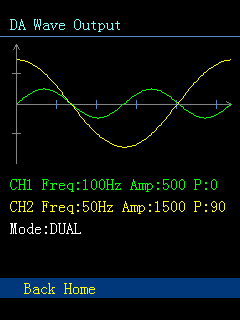
\includegraphics[width=0.42\textwidth]{figures/lcd_dawave.png}
\caption{LCD DA Wave 页面显示效果(DUAL，50\,Hz，Amp 1500，相位 90°；CH1 绿、CH2 黄)}
\label{fig:lcd-da-wave}
\end{figure}

\clearpage

% ==============================
% 第 6 章：电参量计算与分析
% ==============================
\sectiontitle{6}{电参量计算与分析}
\phantomsection\label{sec:calculation}

电参量计算是系统的核心功能之一，将 ADC 采集的原始样点转换为有意义的电气物理量。本章介绍交流电参量计算方法、本系统的程序实现方案以及与上位机的通信设计。

\subsectiontitle{6.1}{交流电参量计算方法}
\phantomsection\label{sec:calculation-method}

交流电参量的计算方法主要有以下三类：

\textbf{(1)直接计算方法。}对采样得到的离散时域信号直接进行数学运算。电压有效值(RMS)定义为 $V_{RMS} = \sqrt{\frac{1}{N}\sum_{i=0}^{N-1}(V_i - V_{dc})^2}$，有功功率定义为 $P = \frac{1}{N}\sum_{i=0}^{N-1} V_i \times I_i$。该方法计算简单、实时性好，对采样率要求不高，适合嵌入式系统。

\textbf{(2)DFT计算方法。}将时域信号变换到频域，提取基波和各次谐波分量。可分别计算各谐波的幅值和相位，进而得到各次谐波功率。计算量为 $O(N^2)$，在样点数较多时开销较大。

\textbf{(3)FFT计算方法。}DFT 的快速算法，计算量 $O(N \log N)$。适合样点数较多(通常要求 2 的幂次)且需要频谱分析的场景。在 Cortex-M3 上实现 FFT 需要额外的运算库。

由于 Cortex-M3 无浮点单元，这里采用整数运算。优点是计算量小、实时性好，且无需复数运算与频谱分析。

\subsectiontitle{6.2}{程序实现}
\phantomsection\label{sec:calculation-program}

电参量计算由 pm\_calc\_electrical() 函数完成。计算流程如下：

\textbf{(1)DC 偏移确定。}为了扣除输入信号叠加的 1.65V 直流偏置，系统实现了零偏自校准算法。在上电启动时，程序采集第一帧（128点，包含完整工频周期）数据并计算其算术平均值作为各通道的直流偏置零点，并在随后的运行中动态扣除，从而有效消除了电阻分压和运放器件失调带来的硬件容差，实现无负载时电压、电流和功率读数的精准归零。

\textbf{(2)RMS 码值计算。}对每通道去直流后计算均方根值：

$$\text{RMS}_{code} = \sqrt{\frac{1}{N}\sum_{i=0}^{N-1}(x_i - Z)^2}$$

中间平方和使用 u64(64 位无符号整数)累加，12 位 ADC 码值的平方最大 $2047^2 \approx 4.19 \times 10^6$，128 点累加最大约 $5.37 \times 10^8$，远小于 u64 上限 $1.84 \times 10^{19}$，不会溢出。开平方运算采用高效的整数开平方算法实现，返回所求平方根的整数部分。

\textbf{(3)物理量换算。}RMS 码值通过校准增益转换为物理量：

$$V_{rms} \times 100 = \text{RMS}_{code} \times G_v / 1000$$
$$I_{rms} \times 1000 = \text{RMS}_{code} \times G_i / 1000$$

其中 $G_v$、$G_i$ 为校准增益$\times$1000。电压通道增益 $G_v = 17600$(对应实际电压互感器与分压比)，电流通道增益 $G_i$ 由实测标定(默认 1000，即 1:1)。电压增益按实测比值整定，可通过修改 \texttt{APP\_ADC\_CALIB\_V\_GAIN\_X1000} 宏调整，无需重新编写算法。特别说明：DAC 环回测试采用单位增益($G_v=1000, G_i=1000$)验证算法趋势，其输出值表现为“去直流RMS码值/100”，此时幅值1500对应的电压值为10.60V；而 miniIO 实际市电测量时则采用校准增益 $G_v = 17600, G_i = 1000$。

\textbf{(4)有功功率计算。}逐点计算去直流后的瞬时功率积并取均值。由于 miniIO 副板 CT1 电流互感器输出极性与电压通道相反，程序中通过配置宏 \texttt{APP\_ADC\_I\_POLARITY = $-$1} 对电流通道的交流分量取反，使普通负载的有功功率显示为正值。该修正仅影响有功功率的符号约定，不影响电压有效值、电流有效值和视在功率的计算结果。修正后的公式为：

$$P_{code} = \frac{1}{N}\sum_{i=0}^{N-1}(v_i - Z_v) \times (i_i - Z_i) \times p_i$$

其中 $p_i$ 为电流通道极性修正系数(默认 $-1$)。有功功率物理量：

$$P \times 10 = P_{code} \times G_v \times G_i / 10^{10}$$

除数为 $10^{10}$ 的原因是 $V_{rms}\times100$(单位 0.01 V)和 $I_{rms}\times1000$(单位 0.001 A)的单位缩放因子不同，$\times$增益$^2$后需除以增益$^2 \times 10000$。结果保留符号，正值表示消耗功率，负值表示回馈功率。

\textbf{(5)视在功率：}$S \times 10 = V_{rms\times100} \times I_{rms\times1000} / 10000$。

\textbf{(6)功率因数：}$\text{PF} \times 1000 = |P| \times 1000 / S$，钳位到 [0, 1000] 区间。$S = 0$ 时(无负载)PF 返回 0，因为无负载时功率因数无物理意义。

% [占位图]
\begin{figure}[H]
\centering
\begin{tikzpicture}[node distance=7mm, >=Latex]
  \node[blk] (p1) {ADC 128 点样点(三通道)};
  \node[blk, below=of p1, align=center] (d) {上电自校准扣除\\各通道直流零偏};
  \node[blk, below=of d] (p2) {去直流 RMS 码值\\$\text{RMS}=\sqrt{\tfrac1N\sum_{i=0}^{N-1}(x_i-Z)^2}$(整数开方)};
  \node[blk, below=of p2] (p3) {物理量换算\\$V_{rms}{\times}100=\text{RMS}\cdot G_v/1000$\\$I_{rms}{\times}1000=\text{RMS}\cdot G_i/1000$};
  \node[blk, below=of p3] (p4) {有功功率\\$P{\times}10=\overline{(v{-}Z_v)(i{-}Z_i){\cdot}p_i}\cdot G_vG_i/10^{10}$\\$p_i$ 为极性修正系数};
  \node[blk, below=of p4] (p5) {视在功率\\$S{\times}10=V_{rms\times100}\cdot I_{rms\times1000}/10^{4}$};
  \node[blk, below=of p5] (p6) {功率因数\\$\text{PF}{\times}1000=|P|\cdot1000/S$，钳位 $[0,1000]$};
  \draw[fl] (p1)--(d);
  \draw[fl] (d)--(p2);
  \draw[fl] (p2)--(p3);
  \draw[fl] (p3)--(p4);
  \draw[fl] (p4)--(p5);
  \draw[fl] (p5)--(p6);
\end{tikzpicture}
\caption{电参量计算流程图}
\label{fig:calc-flow}
\end{figure}

\subsectiontitle{6.3}{通信设计}
\phantomsection\label{sec:calculation-comm}

电参量通过串口协议的 \texttt{STATUS?} 命令和定时自动上报功能传输至上位机，通信协议设计详见第~\ref{sec:protocol-design}~节。

\textbf{自动上报逻辑：}当开启自动上报（通过指令 \texttt{REPORT ON}，见表~\ref{tab:system-commands}）且触发标志 \texttt{take\_report} 置位时，主循环读取最新的全局电参量计算快照，并将其格式化为 STATUS 行，封装为 \texttt{TYPE=0x82} 的事件帧主动推送至上位机。该机制显著降低了上位机的轮询开销，提高了数据吞吐效率。

\clearpage

% ==============================
% 第 7 章：系统调试
% ==============================
\sectiontitle{7}{系统调试}
\phantomsection\label{sec:debug}

本章对系统的串口通信协议、PWM 频率输出、输入捕获测频、ADC 采样、电参量计算以及 miniIO 联机运行进行调试。调试过程采用"命令下发——设备响应——LCD 显示——数据记录——结果分析"的方式进行，重点验证通信协议可靠性、频率测量正确性、ADC 采样稳定性和电参量计算趋势正确性。

\subsectiontitle{7.1}{通信协议测试}
\phantomsection\label{sec:debug-protocol}

本节对系统通信协议设计（见第~\ref{sec:protocol-design}~节）的正确性与可靠性进行调试与测试。主要验证二进制帧的帧头识别、长度解析、命令处理、CRC 校验及协议错误帧拦截等功能。

测试时，上位机通过串口调试工具发送命令帧，观察设备端返回的响应帧及数据流，测试项目与结果记录见表~\ref{tab:protocol-test}。

\begin{table}[H]
\centering
\zihao{-5}
\caption{通信协议测试记录表}
\label{tab:protocol-test}
\begin{tabular}{lllll}
\toprule
测试项目 & 发送命令 & 期望结果 & 实际结果 & 结论 \\
\midrule
帮助命令 & HELP & 返回支持的命令列表 & 返回 4 行命令列表 & 通过 \\
状态查询 & STATUS? & 返回 VRMS、IRMS、P 等状态量 & 单帧返回 VRMS/IRMS/P 等 & 通过 \\
自动上报 & REPORT ON & 周期返回 TYPE=0x82 事件帧 & 每约 1 s 收到一帧 0x82 & 通过 \\
PWM 设置 & PWM SET 50 & PWM 频率更新为 50 Hz & 应答 OK PWM FREQ=50Hz & 通过 \\
DAC 设置 & DAC SET CH1 FREQ 50 & DAC 通道1频率更新为 50 Hz & 应答 OK DAC CH1 FREQ=50Hz & 通过 \\
CRC 错误 & 修改 CRC 字节 & 设备丢弃或返回错误帧 & 翻转末字节后无响应 & 通过 \\
\bottomrule
\end{tabular}
\end{table}

通过测试可见，协议解析器能够正确识别合法帧，并能对异常帧进行过滤或错误响应，满足系统远程参数设置和状态上报需求。

% [占位图]
\begin{figure}[H]
\centering
\begin{lstlisting}[style=serialterm]
$ serial_cmd /dev/cu.usbserial-110 "STATUS?"
>> STATUS?
<< RSP OK STATUS MEAS=50.00Hz PWM=50Hz REPORT=ON DAC_MODE=DUAL DAC_FREQ1=50Hz DAC_FREQ2=50Hz DAC_AMP1=1500 DAC_AMP2=1500 DAC_PHASE1=0 DAC_PHASE2=0 VRMS=10.60 IRMS=1.060 ILK=0.394 P=11.2 S=11.2 PF=1.000

# STATUS? 命令帧(A5 5A 帧头 + CRC-16/Modbus，SEQ=0x2A 示例)
#   A5 5A(SOF) 01(VER) 01(TYPE) 2A(SEQ) 07 00(LEN) 53 54 41 54 55 53 3F("STATUS?") B4 59(CRC)
#   CRC 覆盖 VER..Payload，即 01 01 2A 07 00 53..3F，计算得 B4 59

$ crc_test /dev/cu.usbserial-110
=== 测试 1：正确 CRC 帧 (STATUS?)              收到 1 条响应 -> 正常响应
=== 测试 2：破坏 CRC 帧 (翻转 CRC 末字节)        收到 0 条响应 -> 被正确拒绝(静默丢弃)
=== 测试 3：篡改 payload 保留原 CRC (HELP->HALP)  收到 0 条响应 -> 被正确拒绝
\end{lstlisting}
\caption{串口协议帧与 CRC 校验}
\label{fig:protocol-hex}
\end{figure}

\subsectiontitle{7.2}{频率调试}
\phantomsection\label{sec:debug-frequency}

频率调试采用 PA8/TIM1\_CH1 输出 PWM 方波，PA1/TIM2\_CH2 输入捕获测量频率。调试时将 PA8 与 PA1 短接进行内部环回自测，或使用外部信号源输入 PA1。串口发送 PWM SET 命令修改输出频率，观察串口 STATUS? 返回的 PWM 设定值和 MEAS 测量值，同时记录 LCD 的 Freq Measure 页面显示结果。

\begin{table}[H]
\centering
\zihao{-5}
\caption{频率调试记录表}
\label{tab:pwm-test}
\begin{tabular}{llllllll}
\toprule
目标频率 & 设置命令 & PSC & ARR & 仪器实测 & TIM2 测量值 & 相对误差/\% & 结论 \\
\midrule
50 Hz & PWM SET 50 & 21 & 65454 & 50.0011 Hz & 50.00 Hz & 0.00 & 通过 \\
100 Hz & PWM SET 100 & 10 & 65454 & 100.002 Hz & 100.00 Hz & 0.00 & 通过 \\
1 kHz & PWM SET 1000 & 1 & 35999 & 1000.03 Hz & 1000.00 Hz & 0.00 & 通过 \\
10 kHz & PWM SET 10000 & 0 & 7199 & 10000.3 Hz & 10000.00 Hz & 0.00 & 通过 \\
100 kHz & PWM SET 100000 & 0 & 719 & 100003 Hz & 100000.00 Hz & 0.00 & 通过 \\
\bottomrule
\end{tabular}
\end{table}

表 \ref{tab:pwm-test} 中"仪器实测"栏为 SIGLENT 数字示波器频率计的实测读数，作为外部基准与 TIM2 输入捕获测量值对比。由于 PA8 输出与 PA1 捕获共用 STM32 的同一 72 MHz 时钟，TIM2 测量值与目标频率完全吻合；示波器采用独立时基，其读数与目标的偏差均在 $\pm$0.003\% 以内，二者一致表明频率测量功能正确。

\textbf{超时验证：}断开 PA1 输入信号，观察 2 秒后 LCD 频率显示是否归零。

由测试结果可知，在测试频率范围内，TIM2 输入捕获能够正确反映外部方波频率。TIM2 采用 1 μs 计数分辨率，低频时相对分辨率高。本测试中 PWM 输出与输入捕获共用同一 72 MHz 时钟且分频均为整数，故实测各频点 TIM2 测量值与目标完全一致。对外部非同源信号，高频端单周期测量对计数量化更敏感；如需更高精度，可采用多周期平均法。PWM 频率的软件设定范围为 1--100000 Hz，实际输出波形质量受定时器 PSC/ARR 整数分频、IO 负载、PA8 板载 LED 连接以及测试设备带宽影响，高频端的真实分辨率限制需结合独立时基的示波器或逻辑分析仪实测结果判断。

\begin{figure}[H]
\centering
\begin{subfigure}[t]{0.48\textwidth}
  \centering
  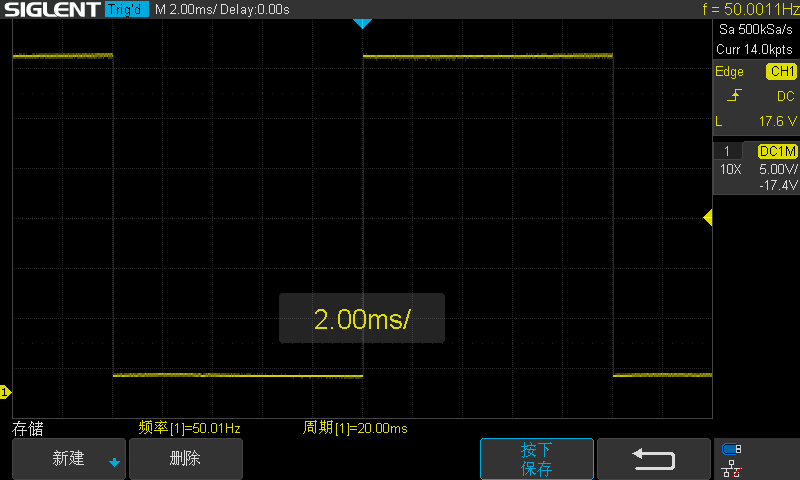
\includegraphics[width=\linewidth]{figures/freq_50hz.png}
  \caption{50 Hz(实测 50.0011 Hz)}
\end{subfigure}
\hfill
\begin{subfigure}[t]{0.48\textwidth}
  \centering
  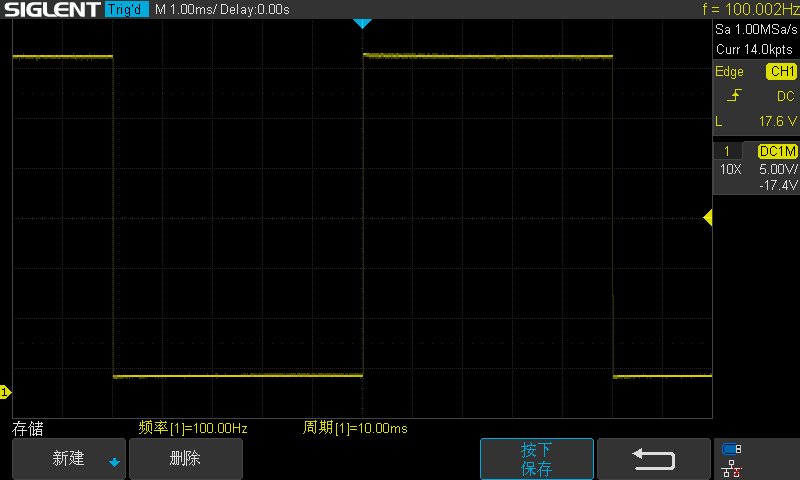
\includegraphics[width=\linewidth]{figures/freq_100hz.png}
  \caption{100 Hz(实测 100.002 Hz)}
\end{subfigure}

\vspace{0.3cm}
\begin{subfigure}[t]{0.48\textwidth}
  \centering
  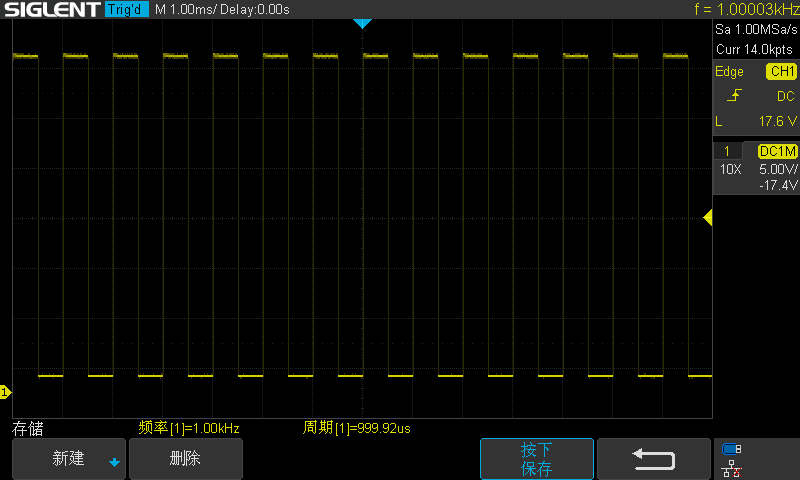
\includegraphics[width=\linewidth]{figures/freq_1khz.png}
  \caption{1 kHz(实测 1.00003 kHz)}
\end{subfigure}
\hfill
\begin{subfigure}[t]{0.48\textwidth}
  \centering
  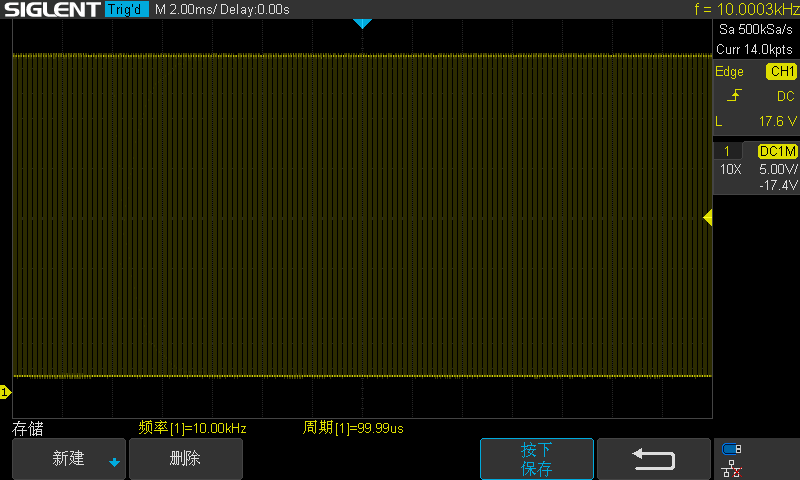
\includegraphics[width=\linewidth]{figures/freq_10khz.png}
  \caption{10 kHz(实测 10.0003 kHz)}
\end{subfigure}

\vspace{0.3cm}
\begin{subfigure}[t]{0.48\textwidth}
  \centering
  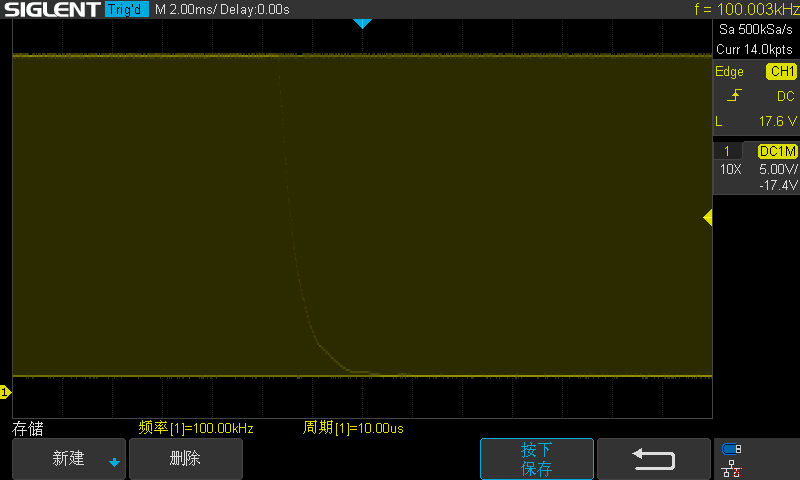
\includegraphics[width=\linewidth]{figures/freq_100khz.png}
  \caption{100 kHz(实测 100.003 kHz)}
\end{subfigure}

\caption{各频率点示波器实测波形(PA8 输出，PA8--PA1 短接环回)}
\label{fig:debug-freq}
\end{figure}

\subsectiontitle{7.3}{AD采样调试}
\phantomsection\label{sec:debug-ad}

ADC 采样调试分为零输入基线测试、DAC 环回测试和波形显示测试。零输入测试时不接外部交流信号，观察 PC0、PC3、PC2 三个 ADC 通道的原始码值是否稳定在中点附近。DAC 环回测试时，将 PA4/DAC\_OUT1 和 PA5/DAC\_OUT2 通过跳线接入 ADC 输入端，设置不同幅值、频率和相位，观察采样结果和电参量变化。

\textbf{(1)零信号基线测试。}不接入外部信号，发送 STATUS? 查看各通道 ADC 原始码值范围。PC0 和 PC3 在无信号时应稳定在中点附近(约 2048)，若某通道码值明显偏大或偏小，说明引脚被外部电路拉偏。

\textbf{(2)DAC 环回测试。}将 DAC 输出(PA4/PA5)通过挑线连接到 ADC 输入(PC0/PC3)，发送 DAC SET MODE DUAL、DAC SET CH1 FREQ 50、DAC SET CH1 AMP 1500 等命令配置测试信号，观察 ADC 采样波形和电参量。理论中点为 2048，实际运行时以上电首帧均值锁定各通道零偏，因此各通道即使静态偏置偏离 2048，也可通过软件去直流后参与 RMS 计算。

\textbf{(3)波形验证。}在 LCD DA Wave 页面观察 DAC 波形预览是否为标准正弦波；在串口查看 VRMS 和 IRMS 值是否与 DAC 幅度设置一致。

\begin{table}[H]
\centering
\zihao{-5}
\caption{ADC 原始采样记录表}
\label{tab:adc-raw}
\begin{tabular}{lllllll}
\toprule
测试条件 & 通道 & 最小值 & 最大值 & 平均值 & 峰峰值 & 结论 \\
\midrule
零输入 & PC0/VL & 2042 & 2057 & 2050 & 15 & 稳定在中点附近 \\
零输入 & PC3/iL & 2049 & 2056 & 2050 & 7 & 稳定在中点附近 \\
零输入 & PC2/iLK & 1943 & 1949 & 1945 & 6 & 稳定在中点附近 \\
DAC 50 Hz AMP=1500 & PC0/VL & 550 & 3550 & 2051 & 3000 & 约 2048 $\pm$ 1500 正弦波 \\
DAC 50 Hz AMP=1500 & PC3/iL & 550 & 3551 & 2050 & 3001 & 约 2048 $\pm$ 1500 正弦波 \\
\bottomrule
\end{tabular}
\end{table}


% [占位图]
\begin{figure}[H]
\centering
\begin{lstlisting}[style=serialterm]
# DAC->ADC 跳线环回 (PA4->PC0, PA5->PC3)
$ serial_cmd /dev/cu.usbserial-110 "DAC SET MODE DUAL"
>> DAC SET MODE DUAL
<< RSP OK DAC MODE=DUAL
$ serial_cmd /dev/cu.usbserial-110 "DAC SET CH1 FREQ 50"
>> DAC SET CH1 FREQ 50
<< RSP OK DAC CH1 FREQ=50Hz
$ serial_cmd /dev/cu.usbserial-110 "DAC SET CH2 FREQ 50"
>> DAC SET CH2 FREQ 50
<< RSP OK DAC CH2 FREQ=50Hz
$ serial_cmd /dev/cu.usbserial-110 "DAC SET CH1 AMP 1500"
>> DAC SET CH1 AMP 1500
<< RSP OK DAC CH1 AMP=1500
$ serial_cmd /dev/cu.usbserial-110 "DAC SET CH2 AMP 1500"
>> DAC SET CH2 AMP 1500
<< RSP OK DAC CH2 AMP=1500
$ serial_cmd /dev/cu.usbserial-110 "STATUS?"
>> STATUS?
<< RSP OK STATUS MEAS=50.00Hz PWM=50Hz REPORT=OFF DAC_MODE=DUAL DAC_FREQ1=50Hz DAC_FREQ2=50Hz DAC_AMP1=1500 DAC_AMP2=1500 DAC_PHASE1=0 DAC_PHASE2=0 VRMS=10.60 IRMS=1.060 ILK=0.394 P=11.2 S=11.2 PF=1.000
# LCD AC Measure 页同步显示相同读数及电压通道原始码范围 (V ADC min/max)
\end{lstlisting}
\caption{ADC 采样调试结果}
\label{fig:debug-adc}
\end{figure}

\subsectiontitle{7.4}{电参量调试}
\phantomsection\label{sec:debug-calculation}

电参量调试主要验证 VRMS、IRMS、有功功率 P、视在功率 S 和功率因数 PF 的计算趋势。由于本系统未使用标准功率源进行标定，本节仅介绍计算逻辑。

\textbf{(1)幅值线性验证。}DAC 两通道频率固定为 50 Hz、相位均设为 0°，使用 \texttt{DAC SET CH1 AMP} 和 \texttt{DAC SET CH2 AMP} 改变 DAC 幅值(500、1000、1500、2000)，记录 VRMS、IRMS、P、S、PF，验证 VRMS 是否随幅值近似线性增长。注：此处 DAC 环回测试采用单位增益验证算法趋势，得到的 VRMS 和 IRMS 相当于归一化后的 '码值/100' 数值，并非乘以市电增益 Gv=17600 后的真实市电电压。

\begin{table}[H]
\centering
\zihao{-5}
\caption{幅值线性测试记录表}
\label{tab:amp-linear}
\setlength{\tabcolsep}{4.5pt}
\begin{tabular}{ccccccccc}
\toprule
DAC 频率 & 幅值码 & 相位差 & \makecell{单位增益\\环回 VRMS/V} & \makecell{单位增益\\环回 IRMS/A} & P/W & S/VA & PF & 现象分析 \\
\midrule
50 Hz & 500 & 0° & 3.53 & 0.353 & 1.2 & 1.2 & 1.000 & 同相 PF=1，P=S \\
50 Hz & 1000 & 0° & 7.07 & 0.706 & 4.9 & 4.9 & 1.000 & V、I 约 2×，P 约 4× \\
50 Hz & 1500 & 0° & 10.60 & 1.060 & 11.2 & 11.2 & 1.000 & V、I 约 3×，P 约 9× \\
50 Hz & 2000 & 0° & 14.11 & 1.399 & 19.7 & 19.7 & 1.000 & V、I 约 4×，P 约 16× \\
\bottomrule
\end{tabular}
\end{table}

\textbf{(2)相位验证。}DAC 两通道频率为 50 Hz、幅值设为 1500，通道1相位固定为 0°，通过 \texttt{DAC SET CH2 PHASE} 分别设置通道2相位为 0°、90°、180°，观察 P 的符号和 PF 的变化趋势。同相时 P $>$ 0(消耗功率)，反相时 P $<$ 0(回馈功率)，正交时 PF 应接近 0。

\begin{table}[H]
\centering
\zihao{-5}
\caption{相位测试记录表}
\label{tab:phase-test}
\begin{tabular}{llllll}
\toprule
DAC 频率 & 幅值码 & 相位差 & P 符号 & PF 理论趋势 & PF 实测值 \\
\midrule
50 Hz & 1500 & 0° & 正 & 接近 1 & 1.000 \\
50 Hz & 1500 & 90° & 接近 0 & 接近 0 & 0.044 \\
50 Hz & 1500 & 180° & 负 & 接近 1 & 1.000 \\
\bottomrule
\end{tabular}
\end{table}

\textbf{(3)无负载情况。}无信号输入时 S = 0，PF 应返回 0(非 NaN 或无穷大)。

\textbf{(4)零信号电平验证。}无信号输入时，由于直流偏置已被固定扣除，各通道的 VRMS 和 IRMS 值应接近 0。

测试结果显示，幅值增大时 VRMS 和 IRMS 随之增大；同相输入时有功功率为正，反相输入时有功功率为负；正交输入时功率因数接近 0，符合交流电参量计算规律。

% [占位图]
\begin{figure}[H]
\centering
\begin{lstlisting}[style=serialterm]
# 幅值线性(DUAL，50 Hz，相位 0)，STATUS? 省略前缀字段
>> DAC SET CH1 AMP 1000
<< RSP OK DAC CH1 AMP=1000
>> DAC SET CH2 AMP 1000
<< RSP OK DAC CH2 AMP=1000
>> STATUS?
<< RSP OK STATUS ... DAC_FREQ1=50Hz DAC_FREQ2=50Hz DAC_AMP1=1000 DAC_AMP2=1000 DAC_PHASE1=0 DAC_PHASE2=0 VRMS=7.07 IRMS=0.706 P=4.9 S=4.9 PF=1.000
>> DAC SET CH1 AMP 1500
<< RSP OK DAC CH1 AMP=1500
>> DAC SET CH2 AMP 1500
<< RSP OK DAC CH2 AMP=1500
>> STATUS?
<< RSP OK STATUS ... DAC_FREQ1=50Hz DAC_FREQ2=50Hz DAC_AMP1=1500 DAC_AMP2=1500 DAC_PHASE1=0 DAC_PHASE2=0 VRMS=10.60 IRMS=1.060 P=11.2 S=11.2 PF=1.000

# 相位(DUAL，50 Hz，幅值 1500)
>> DAC SET CH2 PHASE 90
<< RSP OK DAC CH2 PHASE=90
>> STATUS?
<< RSP OK STATUS ... DAC_FREQ1=50Hz DAC_FREQ2=50Hz DAC_AMP1=1500 DAC_AMP2=1500 DAC_PHASE1=0 DAC_PHASE2=90 VRMS=10.60 IRMS=1.060 P=0.5 S=11.2 PF=0.044
>> DAC SET CH2 PHASE 180
<< RSP OK DAC CH2 PHASE=180
>> STATUS?
<< RSP OK STATUS ... DAC_FREQ1=50Hz DAC_FREQ2=50Hz DAC_AMP1=1500 DAC_AMP2=1500 DAC_PHASE1=0 DAC_PHASE2=180 VRMS=10.60 IRMS=1.060 P=-11.2 S=11.2 PF=1.000
\end{lstlisting}
\caption{电参量调试结果}
\label{fig:debug-calc}
\end{figure}

\subsectiontitle{7.5}{联机调试}
\phantomsection\label{sec:debug-online}

联机调试将 MiniSTM32 开发板通过串口连接上位机，同时观察 LCD 显示和串口数据。调试分为 DAC 环回测试和 miniIO 实际接入测试两部分。MiniSTM32 开发板通过 CH340 USB 转串口芯片连接上位机 USB 口，串口配置 115200 8N1。

\textbf{(1)DAC 环回测试。}将 PA4/DAC\_OUT1、PA5/DAC\_OUT2 通过跳线连接至 ADC 输入端，用于验证 ADC 采样、DMA 数据拆分、电参量计算和串口上报功能。该模式不接入市电，便于调整正弦波幅值、频率和相位，并观察 VRMS、IRMS、P、S、PF 等参数是否随输入信号变化。

\textbf{(2)miniIO 实际接入测试。}MiniSTM32 与 miniIO 通过 JP1 排线连接(接线关系见图~\ref{fig:miniio-connect})。负载接入 miniIO 的交流输入输出端后，系统通过 ADC 采集电压、电流和漏电电流信号，通过 TIM2 输入捕获测量市电频率，并在 LCD 与串口 STATUS 数据中显示计算结果。联机调试时需同时记录 miniSTM32 与 miniIO 接线图、LCD 显示页面、串口助手返回数据和若干组稳定性测试数据。

\textbf{联机验证内容：}

(1)上电后串口收到事件帧 ``OK COURSE1 READY''，确认固件启动正常。

(2)LCD 显示 Dashboard 仪表盘页面(默认首页)，通过 KEYUP(上)/KEY1(下)/KEY0(确认)导航各子页面，确认 LCD 渲染正确。

(3)通过串口发送各命令，验证响应帧内容正确、CRC 校验通过。

(4)开启 REPORT ON，观察自动上报数据流是否按约 1 秒周期稳定推送。

(5)对比 LCD 显示数值和串口 STATUS? 查询结果，确认两端数据一致。

联机运行后，串口发送 STATUS? 获取系统状态，并与 LCD 页面显示结果对比。若两端 VRMS、IRMS、P、S、PF 和频率显示一致，说明 LCD 和串口均读取同一全局状态数据，数据链路保持一致。开启 REPORT ON 后，在 DAC 环回测试环境下进行长时间连续运行，记录稳定性数据如表 \ref{tab:stability-test} 所示。

\begin{table}[H]
\centering
\zihao{-5}
\caption{系统联调稳定性测试记录表 (DAC 环回模式)}
\label{tab:stability-test}
\begin{tabular}{llllll}
\toprule
测试时间 & 上报周期 & 串口异常次数 & LCD 刷新 & 数据波动范围 & 结论 \\
\midrule
1 min & 1 s & 0 & 正常 & VRMS 10.60--10.61 V & 稳定，无丢帧 \\
3 min & 1 s & 0 & 正常 & VRMS 10.60--10.61 V & 稳定，无丢帧 \\
5 min & 1 s & 0 & 正常 & VRMS 10.60--10.61 V & 稳定，无丢帧 \\
\bottomrule
\end{tabular}
\end{table}

% [占位图]
\begin{figure}[H]
\centering
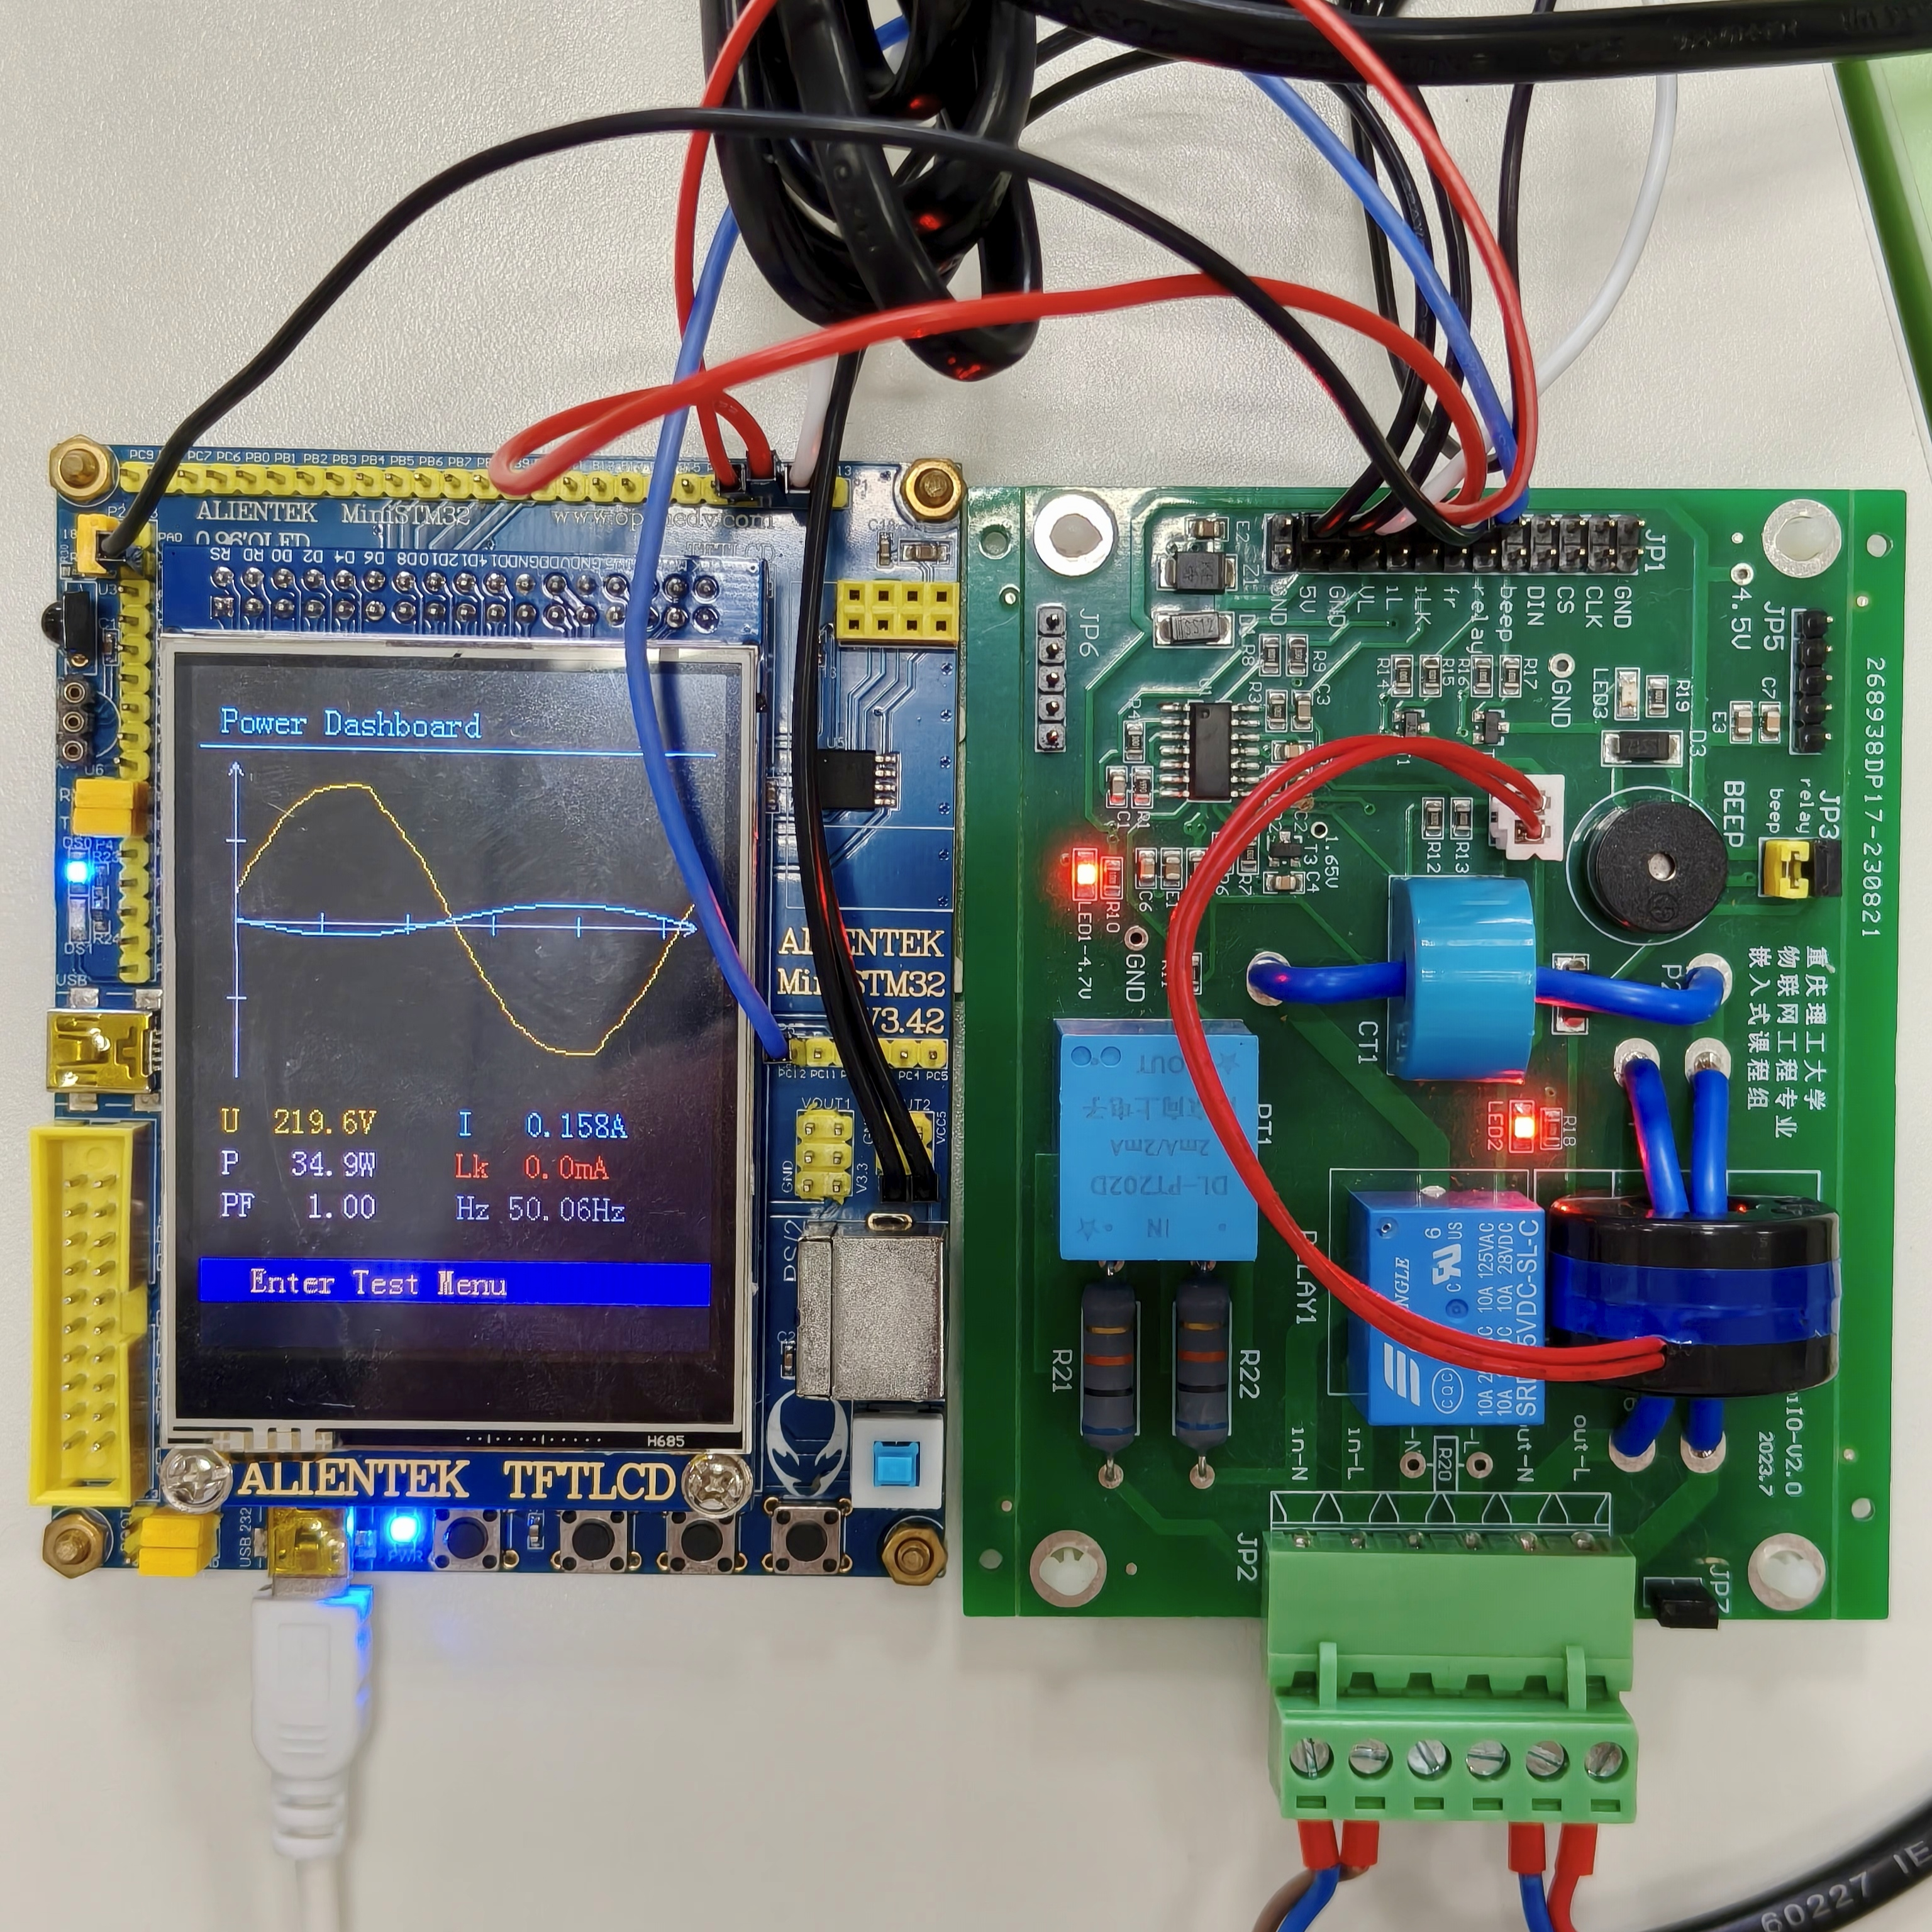
\includegraphics[width=0.9\linewidth]{figures/debug_online_actual.jpg}
\caption{miniSTM32 与 miniIO 接线实物图}
\label{fig:debug-online}
\end{figure}

% [占位图]
\begin{figure}[H]
\centering
\begin{subfigure}[t]{0.30\textwidth}
  \centering
  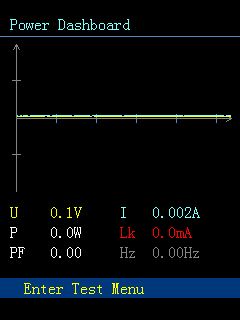
\includegraphics[width=\linewidth]{figures/lcd_dashboard.png}
  \caption{首页仪表盘}
\end{subfigure}
\hfill
\begin{subfigure}[t]{0.30\textwidth}
  \centering
  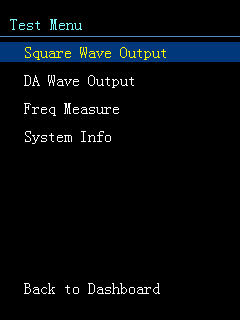
\includegraphics[width=\linewidth]{figures/lcd_testmenu.png}
  \caption{调试菜单}
\end{subfigure}
\hfill
\begin{subfigure}[t]{0.30\textwidth}
  \centering
  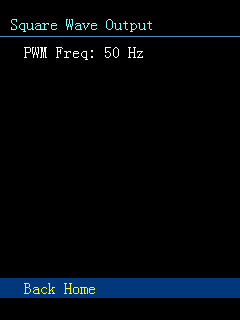
\includegraphics[width=\linewidth]{figures/lcd_square.png}
  \caption{方波输出页}
\end{subfigure}

\vspace{0.3cm}
\begin{subfigure}[t]{0.30\textwidth}
  \centering
  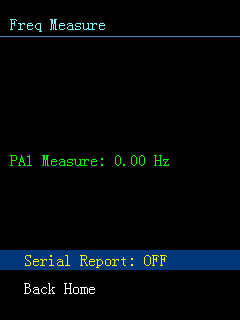
\includegraphics[width=\linewidth]{figures/lcd_measure.png}
  \caption{频率测量页}
\end{subfigure}
\hfill
\begin{subfigure}[t]{0.30\textwidth}
  \centering
  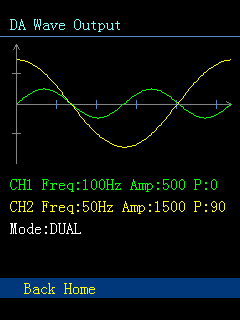
\includegraphics[width=\linewidth]{figures/lcd_dawave.png}
  \caption{DA 波形输出页}
\end{subfigure}
\hfill
\begin{subfigure}[t]{0.30\textwidth}
  \centering
  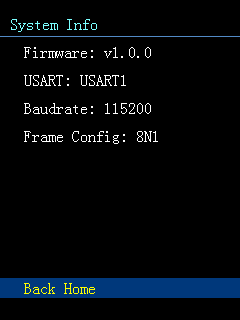
\includegraphics[width=\linewidth]{figures/lcd_info.png}
  \caption{系统信息页}
\end{subfigure}
\caption{LCD 各页面显示效果}
\label{fig:lcd-pages}
\end{figure}

\clearpage

% ==============================
% 第 8 章：总结与展望
% ==============================
\sectiontitle{8}{总结与展望}
\phantomsection\label{sec:summary}

本次课程设计完成了基于 STM32F103RCT6 的桌面用电监控系统：信号生成、频率测量、DAC 输出、ADC 采样、电参量计算、LCD 显示与串口通信各模块均已实现并联调通过。系统采用前后台多任务轮询结构，无 RTOS 依赖，软件分层清晰，LCD 显示与串口查询通过全局状态数据保持数据一致。

\textbf{调试过程中遇到的主要问题及解决办法：}

(1)PC1(ADC1\_IN11)电流通道读数异常。现象：DAC DUAL 环回测试时 IRMS 始终约为 0.056，远小于预期。排查发现 MiniSTM32 开发板的 PC1 与触摸屏 PEN/控制线相关并存在上拉影响，硬件上拉电阻将 PC1 拉至约 3V，导致 ADC 读数严重偏高。解决办法：将电流采样通道迁移至 PC3(ADC1\_IN13)，避开触摸屏干扰。

(2)ADC 采样数据竞争。现象：LCD 显示的电参量偶尔跳变，与串口 STATUS 返回的数据不一致。根因是 DMA ISR 正在写入缓冲区时主循环同时在读取。解决办法：根据 AI 工具的建议，设计了三重缓冲数据隔离机制——中断写双缓冲、主循环在极短临界区内提取就绪帧号，计算完毕后复制到显示缓冲帧，解决了数据不一致问题。

(3)继电器控制异常。现象：联机后继电器无法正确吸合，导致无法测得实际市电参数。排查发现初始化函数 \texttt{app\_init()} 中遗漏了对 \texttt{app\_relay\_init()} 的调用，导致 PC12 引脚未被配置。解决办法：在 \texttt{app\_init()} 中补全继电器初始化调用，确保上电默认安全断开，并在切入 Dashboard 仪表盘页时正确吸合。

(4)有功功率初始为负值。现象：普通负载接入后，电流、视在功率和有功功率幅值均随负载变化正常，但有功功率始终显示为负值。排查发现 miniIO 副板 CT1 电流互感器的输出极性与电压通道传感器相反，导致软件按默认极性计算时电流信号相对电压信号反相，有功功率符号取反。解决办法：在配置文件中引入电流通道极性修正宏 \texttt{APP\_ADC\_I\_POLARITY}，默认值为 $-1$，在有功功率计算中对电流通道的去直流分量取反。

\textbf{心得体会：}

本次课程设计中最具挑战性的部分是数据竞争问题的排查——DMA 中断与主循环并发访问同一缓冲区的问题在代码审查中难以发现，需要结合现象反复推理数据时序。三重缓冲隔离机制的设计过程加深了我对嵌入式并发数据一致性的理解。

在团队协作方面，小组成员针对引脚分配、协议帧格式以及滤波算法的选择展开了充分讨论，通过将系统配置常量集中定义于 \texttt{app\_config.h}、协议帧结构规范化定义于 \texttt{app\_protocol\_defs.h}，有效保障了下位机固件与上位机分析工具之间的通信一致性。在调试及分析过程中，AI辅助工具在架构优化，分析数据竞争等复杂问题上提供了有益的指导，但针对菜单界面设计、交互逻辑、需求分析和具体的硬件寄存器操作、引脚分配问题，仍需人工进行规划、审查与测试验证。例如 PC1 电流通道读数异常的问题，需要人工查阅开发板资料并正确规划引脚分配。

\textbf{改进方向：}

(1)增加 FFT 频谱分析功能，支持谐波检测。

(2)优化串口协议，支持批量数据传输，便于绘制实时波形。

(3)优化 LCD 显示效果，采用增量刷新等策略以减少屏幕闪烁。

\end{document}
